\chapter[Objetos Relevantes]{Objetos y Fenómenos Astrofísicos Relevantes}
\thispagestyle{empty}
\section{Nubes Moleculares Gigantes}

Las grandes ``guarderías'' de estrellas a lo largo de la Galaxia se localizan en nubes moleculares gigantes, compuestas principalmente por hidrógeno molecular $\mathrm{H_2}$.
Siendo que esta molécula solo emite radiación en ultravioleta, donde el medio interestelar tiene una alta extinción, para detectar la presencia de las nubes moleculares se recurre a otras moléculas llamadas ``trazadoras'', principalmente $\mathrm{CO}$, la segunda molécula más abundante en el medio interestelar, que posee líneas espectrales en el rango de las ondas de radio.

Complejos aomo el de Taurus-Auriga se formaron debido a la convergencia de dos flujos de material neutro \citep{Ballesteros:1999} que se enfrió y se volvió más denso debido a inestabilidades térmicas \citep{Hennebelle:1999}. Muchas de estas nubes moleculares tienen forma filamentaria debido a que se están colapsando gravitacionalmente en caida libre \citep{Ballesteros:2011}. Dentro de los filamentos puede haber colapsos locales que pueden dar lugar a regiones de formación estelar de baja masa o incluso asociaciones OB como es el caso de la Nebulosa de Orión \citep{Hartmann:2007}.

\section[Regiones \Ion{H}{II}]{Regiones \Ion{H}{II} \citep{Stahler:2004}}
\label{sec:HII}
\newcommand\Nio{\ensuremath{\mathcal{N}}}
%\newcommand\N{\ensuremath{\mathcal{N}}}

Consideremos el caso en que se forma una estrella masiva dentro de una nube molecular, que por simplicidad está compuesta exclusivamente de hidrógeno molecular $\mathrm{H_2}$. La estrella masiva emite fotones ultravioleta que tienen la energía suficiente para disociar el $\mathrm{H_2}$  como para ionizar el hidrógeno atómico resultante. Luego el plasma ionizado se recombina para volver a ser \Ion{H}{I} emitiendo líneas espectrales de diversas energías, siendo la más energética la línea de \Ion{Ly}{\alpha}. Como al realizar una ionización se pierde un fotón ionizante y el flujo de radiación proveniente de la estrella es finito, entonces la estrella solo puede ionizar la región de la nube más próxima a ésta. Si suponemos que la nube tiene densidad uniforme, entonces esta región tendrá forma esférica, conocida como \textit{esfera de Strömgren}.

\subsection{Esfera de Strömgren}

El plasma ionizado dentro de la Esfera de Strömgren se encuentra en balance de ionización, esto es, que la tasas de ionización y la de recombinación son iguales. La tasa de ionizaciones es igual a la cantidad de fotones ionizantes que emite la estrella central por segundo. Esto es, los fotones que poseen una energía mayor al límite de Lymann, que corresponde a  $E = \SI{13.6}{eV}$, o bien $\lambda = \SI{912}{\angstrom}$. En la tabla \ref{tab:ionizing-radiation} se muestra la tasa de fotones ionizantes $\Nio_*$ para estrellas masivas de tipo espectral O y B temprano.

\begin{table}
  \begin{tabular}{cccc} \toprule
    Tipo & Masa & $\log \Nio_*$ & $\log \Nio_{FUV}$ \\
    Espectral & (\SI{}{M_\odot}) & (\SI{}{s^{-1}}) & (\SI{}{s^{-1}})  \\
    \midrule
    O4 & 70 & 49.9 & 49.5 \\
    O5 & 60 & 49.4 & 49.2 \\
    O6 & 40 & 48.8 & 48.8 \\
    O7 & 30 & 48.5 & 48.6 \\
    O8 & 23 & 48.2 & 48.4 \\
    O9 & 20 & 47.8 & 48.2 \\
    B0 & 18 & 47.1 & 48.1 \\
    B1 & 13 & 45.4 & 47.5 \\
    B2 & 10 & 44.8 & 47.1 \\
    \bottomrule
  \end{tabular}
  \caption{Tasa de fotones ionizantes para estrellas masivas \citep{Stahler:2004}}
  \label{tab:ionizing-radiation}
\end{table}

El radio de esta esfera se denomina \textit{Radio de Strömgren} que viene dado por:


\begin{align}
  R_s = \left[\frac{3\Nio_*}{4\pi\alpha'_{rec}(n^0_H)^2}\right]^{1/3} = 0.4\mathrm{~pc}\left(\frac{\Nio_*}{10^{49}\mathrm{~s^{-1}}}\right)^{1/3}\left(n_{H_2}\right)^{-2/3} \label{eq:stromgren}
\end{align}

Donde $\alpha'_{rec}$ es el coeficiente de recombinación a todos los niveles energéticos del hidrógeno excepto el estado base, $n^0_H$ y $n_{H_2}$ son la densidad numérica del hidrógeno neutro y del hidrógeno molecular donde está embebida la región HII, respectivamente.

En la expresión numérica, se adopta una temperatura de $10^4\mathrm{~K}$ que es la temperatura característica de una región \Ion{H}{II} y con la que el coeficiente de recombinación $\alpha'_{rec}$ adopta un valor de \SI{2.6e-13}{cm^3.s^{-1}}.

Dentro de la región \Ion{H}{II}, la probabilidad por unidad de tiempo de ionizar un átomo de hidrógeno dado es mucho mayor a la probabilidad de una recombinación, por lo que el gas está casi completamente ionizado. Sin embargo, en los bordes la densidad de gas neutro aumenta debido a que en dicha región el flujo de fotones ionizantes ha sido atenuado por todo el gas ionizado más próximo a la estrella. La transición de gas ionizado a gas neutro tiene un grosor $\Delta r$ que corresponde al camino libre medio del gas neutro. Esto es:

\begin{align}
\Delta R = \frac{1}{\sigma_{\nu_1}n^0_H}  
\end{align}

Donde $\sigma_{\nu_1}$ es la sección recta de un átomo de hidrógeno en el estado base, evaluada en la longitud de onda del límite de Lymann. Utilizando $\sigma_{\nu_1} = \SI{6.8e-18}{cm^2}$ y $n^0_H = \SI{2e3} 10^{3}{cm^{-3}}$ obtenemos que $\Delta r = \SI{7.4e13}{cm} \sim \SI{5e-5}{R_s}$, lo que muestra que las regiones \Ion{H}{II} tienden a tener bordes bien delimitados.

Sin embargo, las esferas de Strömgren no son objetos estáticos, sino que se expanden con el tiempo. Este proceso ocurre en dos etapas: en la primera inicialmente no existe ninguna región \Ion{H}{II} pero que la radiación ultravioleta de la estrella hace que se expanda de manera exponencial al disociar e ionizar el gas a su alrededor hasta alcanzar el radio de Strömgren. Posteriormente la diferencia de presiones entre el gas ionizado de la región \Ion{H}{II} y del gas neutro circundante, provoca una segunda expansión con forma de ley de potencias hasta alcanzar equilibrio de presiones.

\subsection{Flujos de Champaña}
La segunda expansión lleva a que la región \Ion{H}{II} se expanda dos órdenes de magnitud por encima del radio de Strömgren, pero el tiempo que toma alcanzar dichas dimensiones es tan largo que la estrella central muere antes de se alcanze el equilibrio de presiones. Sin embargo, es más probable que el frente de ionización rebase el borde de la nube molecular donde se formó, y en este caso el gas ionizado altamente presurizado escapa directamente hacia el medio interestelar que lo rodea (que tiene una presión aún menor que la de la nube molecular), creando el \textit{Flujo de champaña}.

\subsection{Características de la emisión}

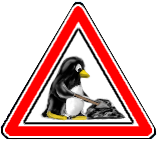
\includegraphics[width=0.1\linewidth]{./Figures/tux-development}


\section{La Nebulosa de Orión}

\begin{figure*}
    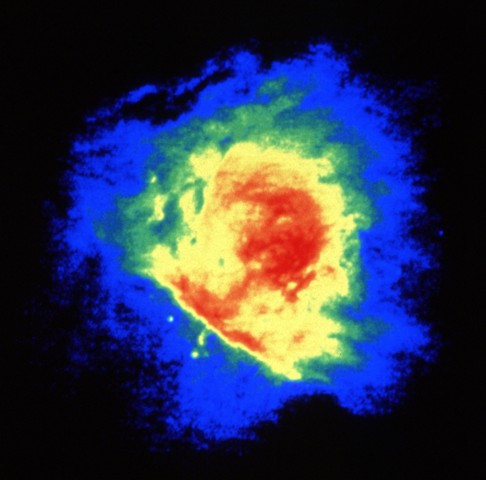
\includegraphics[width=0.5\linewidth]{./Figures/OrionVR13A} 
  \caption{La Nebulosa de Orión observada por el VLA en la banda L ($\lambda = \SI{20}{cm}$, $\nu = \SI{1.4}{GHz}$, \citet{Yusef:1990}).}
\end{figure*}

La Nebulosa de Orión (ONC por sus siglas en inglés), ubicada a $\sim \SI{414}{pc}$ \citep{Menten:2007}, es probablemente la región \Ion{H}{II} mejor estudiada del cielo (ver \S \ref{sec:HII}). Forma parte de la nube molecular gigante de Orión, de donde se distinguen dos sub-unidades, llamadas Orión A y Orión B. ONC forma parte de Orión A. El cúmulo de estrellas que se formó y que es responsable de la región \Ion{H}{II} se conoce como asociación OB Ori Id, cuyos miembros más prominentes son un grupo de cuatro estrellas conocidas como el ``Trapecio''. La más masiva de éstas es \thC{}, de clasificación espectral O6 aproximadamente (ver tabla ), tiene una luminosidad de \SI{4e5}{L_\odot} y una temperatura de \SI{4e4}{K}. Cuando la región \Ion{H}{II} se encuentra embebida en el gas molecular,  no puede ser visible en el rango óptico del espectro. En el caso de ONC, que se ubica cerca del borde de la nube molecular Orion A, el gas ionizado caliente, que posee una presión mayor que el gas molecular frío, se escapa hacia el gas adyacente a la nube molecular en forma de ``flujo de champaña'' (figura \ref{fig:champagne}), y de esta manera el gas ionizado puede ser visible por medio de diferentes líneas espectrales, tanto de hidrógeno como de otros elementos. 

\begin{figure}
  \begin{tabular}{lr}
    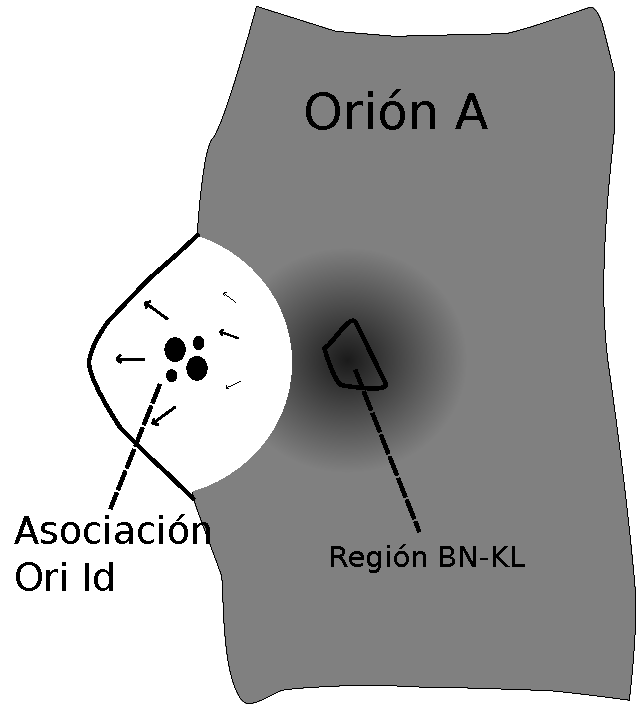
\includegraphics[width=0.4\linewidth]{./Figures/champagne} &
    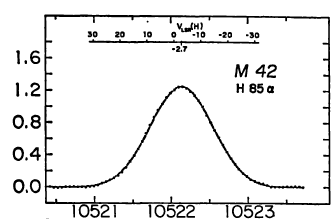
\includegraphics[width=0.5\linewidth]{./Figures/H85-alpha}
    \end{tabular}
  \caption{Izquierda:Representación esquemática de la Asociación Ori Id y su ubicación dentro de la nube molecular gigante Orión A. La región BN-KL es una región de formación estelar muy activa donde se observan entre otras cosas, máseres de agua y SiO y flujos moleculares \citep{Stahler:2004}. Derecha: Línea espectral $H~85~\alpha$ de hidrógeno de ONC. El eje horizontal corresponde a la frecuencia en MHz, mientras que el eje verical representa la temperatura de antena. El espectro muestra un corrimiento al azul que muesta que el gas se acerca a una velocidad de $\sim 3\mathrm{~km~s^{-1}}$ \citep{Stahler:2004, Churchwell:1970}}
  \label{fig:champagne}
\end{figure}

\section{Proplyds}
\subsection{Descubrimiento}
Observaciones en óptico de la región del trapecio en filtros de banda angosta de diferentes líneas de emisión tales como \Ion{H}{\alpha}, \Ion{H}{\beta}, [\Ion{O}{III}], [\Ion{N}{II}], [\Ion{S}{II}] y continuo, revelaron la existencia de objetos puntuales únicamente visibles en líneas de alta ionización (\Ion{H}{\alpha}, \Ion{H}{\beta} y [\Ion{O}{III}]) que fueron inicialmente denominados como ``condensaciones nebulares'' \citep{Laques:1979}. Hasta el momento no se sabía con certeza si ``condensaciones nebulares'' eran en realidad condensaciones nebulares (regiones donde la densidad de la nebulosa es inusualmente alta por alguna razón o bien esferas de gas molecular cuya envolvente fue ionizada y que la radiación de la estrella central la está ``erosionando'') o si se trataba de protoestrellas de baja masa cuyo disco protoplanetario estaba siendo fotoevaporado por la estrella central \citep{churchwell:1987}. No fue sino hasta que se contó con observaciones de alta resolución con el Telescopio Espacial Hubble (HST) que se se pudo determinar la verdadera naturaleza de estos objetos \citep{ODell:1993} y la razón por la que se les denominó ``proplyds'' (PROtoPLanetarY DiskS). A su vez se encontraron por primera vez arcos delgados y otras estructuras de gran interés.

\subsection{¿Qué es un proplyd? Breve introducción \citep{Johnstone:1998}}

Las imágenes del HST de la Nebulosa de Orión mostraron imágenes de discos alrededor de estrellas jóvenes de baja masa. Algnuos se ven como siluetas oscuras que contrastan con la nebulosa, y otros casos son visibles en líneas de emisión de líneas de alta ionización. Un proplyd típico tiene forma cometaria, con una cabeza brillante que apunta hacia la fuente de radiación ionizante, y una cola que se extiende en dirección contraria a ésta. La explicación a esta forma es que el disco protoplanetario está siendo fotoevaporado por la radiación ionizante de una estrella masiva (\thC{} en caso de la Nebulosa de Orión), la cabeza es un frente de ionización cuyo radio escala como $R_{IF} \propto D^{2/3}$, donde $D$ es la distancia a la estrella masiva. La forma de la cola se debe a radiación ionizante difusa, producto de dispersión por polvo y por recombinaciones (Figura \ref{fig:prop-shape}). \citet{churchwell:1987} ya había notado que la tasa de pérdida de masa observada
en el gas ionizado implicaba que la fuente de este gas debía oscurecer a la protoestrella huésped, a menos que proviniera de un disco circumestelar. De la
emisión de radio observada, se estima la densidad electrónica en $n_e \sim \SI{e6}{cm^{-3}}$ y la tasa de pérdida de masa en $\dot{M} \sim \SI{e-7}{M_\odot.yr^{-1}}$.

\begin{figure}
  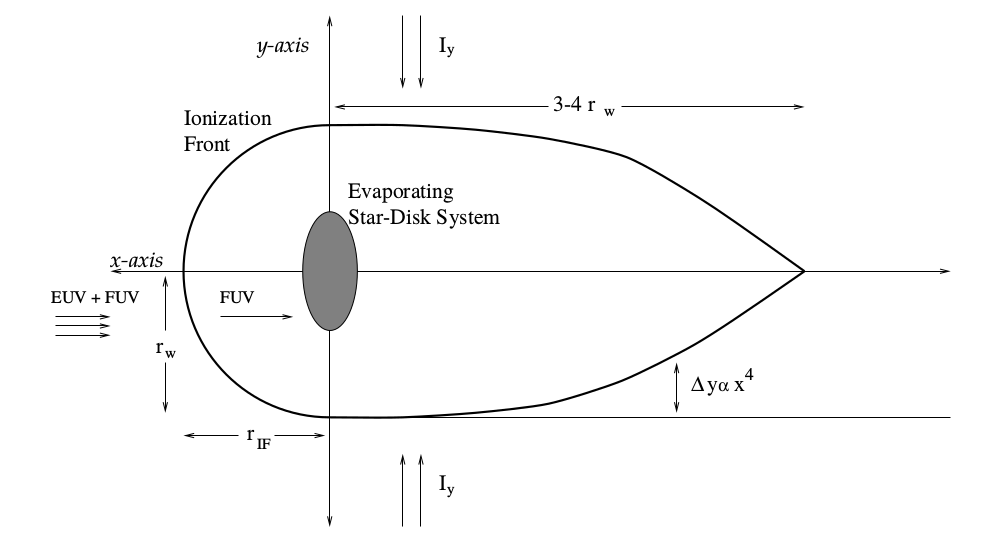
\includegraphics[width=0.8\linewidth]{./Figures/Johnstone-shape}
  \caption{Representación esquemática de la formación de un frente de ionización hemisférico y de una cola de gas ionizado detrás del disco en proceso de fotoevaporación. $r_{IF}$ y $r_w$ representan el radio del frente de ionización en las direcciones de los ejes $x$ e $y$, respectivamente. $I_y$ representa el campo de radiación difusa. Por detrás del disco, la radiación difusa calienta el gas del disco provocando otro flujo fotoevaporado. $\Delta y$ es la diferencia entre la forma actual del frente de ionización por detrás del disco y una forma cilíndrica. La forma de la colase explica como que el flujo de radiación $I_y$ es capaz de penetrar más cerca del eje $x$ conforme uno se aleja del disco, donde el flujo fotoevaporado es menos denso.}
    \label{fig:prop-shape}
\end{figure}


\subsection{Mecanismos de fotoevaporación \citep{Johnstone:1998}}

El principal mecanismo de fotoevaporación es el campo de radiación de la estrella central, en la parte ultravioleta del espectro electromagnético. Según la masa de la estrella central, podemos tener dos clases de flujo radiativo: Dominado por el ultravioleta lejano (FUV, $h\nu < \SI{13.6}{eV}$) o dominado por el ultravioleta extremo (EUV, $h\nu \geq \SI{13.6}{eV}$). En general, el FUV se encarga de disociar moléculas y de calentar el gas de la región de fotodisociación (PDR) hasta temperaturas de \SI{100}{} - \SI{1000}{K}, mientras que el EUV puede ionizar el gas y elevar su temperatura hasta \SI{e4}{K}. El EUV no puede atravesar el frente de ionización (IF) pero el FUV sí.

En el caso de que el flujo sea dominado por el EUV, la presión térmica del flujo fotoevaporado es determinada por la fotoionización, la PDR producida por el FUV es delgada. El gas calentado por el FUV se mueve de manera subsónica hasta llegar al IF y la tasa de pérdida de masa depende de la tasa de ionización inducida por el EUV.

Si el flujo está dominado por el FUV, la presión térmica depende del calentamiento por el FUV. El gas tibio se expande como un viento que empuja el IF lejos del disco. La tasa de pérdida de masa la determina la temperatura de la PDR, el flujo FUV y la opacidad del polvo a las longitudes de onda del FUV. Inicialmente la forma del disco impone una geometría cilíndrica en el flujo fotoevaporado, pero eventualmente los gradiente de presión tornan esta geometría en esférica.

Las ecuaciones de continuidad de la masa y el momento restringen la velocidad del flujo neutro antes de alcanzar el IF. Mas allá de éste, la presión del gas hace que éste se expanda a velocidades del orden de una a dos veces la velocidad del sonido. Para el gas neutro dentro del IF hay dos posibles soluciones: si el gas neutro es supersónico entonces el IF será de baja densidad (Tipo R) con bajo contraste de densidad entre gas neutro y gas ionizado. O si el gas neutro es subsónico se formará un IF tipo D con un gran contraste de densidad entre el gas neutro y el gas ionizado. Sin embargo, sin importar qué tipo de radiación domina la fotoevaporación, el gas neutro permanece a velocidades subsónicas al llegar al IF, por lo que dicho frente será tipo D. En el caso de un flujo dominado por el EUV, el gas neutro permanece a velocidad subsónica, su velocidad decae como $v_I \propto r^{-2}$ y llega a \SI{0.5}{km.s^{-1}} al llegar al frente de ionización. Cundo el flujo es dominado por el FUV, el gas neutro se acelera hasta llegar a velocidades supersónicas, luego atraviesa un choque isotérmico que lo desacelera y llega al frente de ionizacion a \SI{0.5}{km.s^{-1}}.

  \begin{figure}
    \begin{tabular}{cc}
      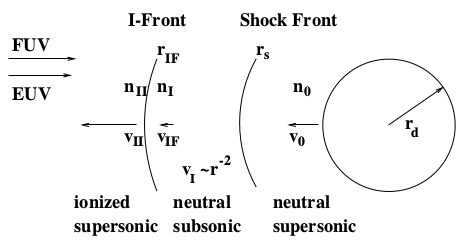
\includegraphics[width=0.5\linewidth]{./Figures/Johnstone-2} &
      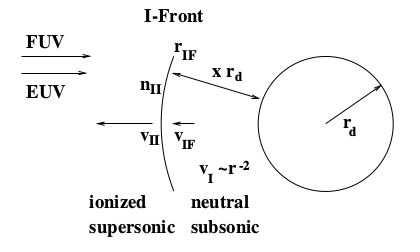
\includegraphics[width=0.5\linewidth]{./Figures/Johnstone-3}
    \end{tabular}
    \label{fig:EUV-FUV-IF}
    \caption{Representación esquemática de las regiones del flujo fotoevaporado de un proplyd. Izquierda: Cuando el flujo es dominado por el FUV. Derecha: Flujo dominado por EUV \citep{Johnstone:1998}}
  \end{figure}
  

Sin importar el tipo de mecanismo de fotoevaporación dominante, el flujo fotoevaporado solo si la presión térmica supera a la gravedad de la protoestrella. Entonces, el flujo fotoevaporado solo existe a partir de un radio crítico $r_g$, donde este radio se estima a partir del balance entre la energía necesaria para escapar de una órbita kepleriana y la energía térmica:
\begin{align}
  r_g = \frac{GM_*}{a^2}
\end{align}
Donde $M_*$ es la masa de la protoestrella y $a$ es la velocidad del sonido del gas. Para las protoestrellas típicas del trapecio la masa típica es de
$M_* = 0.2~M_\odot$. Para el gas neutro la velocidad del sonido es de $a_I \sim \SI{3}{km.s^{-1}}$ y para el gas ionizado es de $a_{II} \sim \SI{10}{km.s^{-1}}$.
Por tanto, el radio gravitacional para un flujo dominado por el EUV es de $r_{gII} \sim \SI{2}{AU}$ y para un flujo dominado por el FUV es de $r_{gI} \sim \SI{20}{AU}$.
\section{Objetos LL}

El arquetipo de esta clase de objetos es LL\,Ori (LL1 de aquí en adelante), son llamados también choques ``in situ'' \citep{Kobulnicky:2016}, donde el choque se da cuando viento de una estrella interactúa con un flujo tal como un flujo de champaña. Sin embargo, no es del todo claro el tipo de flujo interno proveniente de la estrell central (figura \ref{fig:LL-scheme}). \citet{Gutierrez-Soto:2015a} hizo un catálogo de objetos dentro de ONC en los que se observan choques de proa, algunos de ellos no habían sido identificados previamente, a la vez que se realizaron mediciones de $(R'_0, R'_c)$ de cada objeto (ver \S \ref{sec:fundamental-parameters}, \ref{sec:projection}). En las figuras \ref{fig:Luis-mosaic-1} y \ref{fig:Luis-mosaic-2} mostramos algunos ejemplos de este catálogo. A diferencia de los choques de proa más próximos a \thC{}, los choques más exteriores pueden presentar dos cáscaras. Si ese es el caso, los radios $(R'_0, R'_c)$ fueron medidos para ambas cáscaras, así como el grosor $H'$ que es la diferencia de $R'_0$ de ambas cáscaras y la orientación (figura \ref{fig:methodology-LL}).

\begin{figure}
  \includegraphics[width=\linewidth]{./Figures/LL-outer-inner-extend-Luis}
  \caption{Posibiles escenarios para los flujos en interacción de los choques de proa en ONC. Izquierda: Un flujo de champaña transónico interactúa ya sea con el flujo fotoevaporado de un proplyd o con un viento estelar, este caso aplica para los arcos más alejados de \thC{}. Derecha: El viento estelar proveniente de una estrella tipo O interactúa con el flujo fotoevaporado de un proplyd. Aplica para los proplyds más cercanos a \thC{}.}
  \label{fig:LL-scheme}
\end{figure}

\begin{figure}
  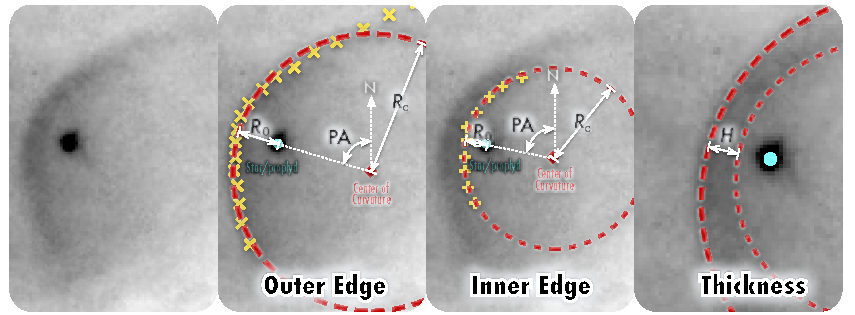
\includegraphics[width=0.7\linewidth]{./Figures/radius-methodology-Luis}
  \caption{Metodología para la medición de los radios característicos $(R'_0, R'_c)$. Para un arco dado, se traza la posición de las dos cáscaras utilizando marcas con el programa DS9 para imágenes astronómicas (las cruces en la figura). Posteriormente, con un ajuste de mínimos cuadrados se ajusta un círculo a las marcas de cada cáscara para obtener el radio de curvatura aparente $R'_c$ (línea roja rayada). $R'_0$ se obtiene como la distancia mínima entre la posición de la estrella y el ajuste circular y por último el grosor $H'$ se obtiene como la diferencia entre ambas mediciones de $R'_0$, suponiendo que estén disponibles.}
  \label{fig:methodology-LL}
\end{figure}

\begin{figure}
  \begin{tabular}{cc}
    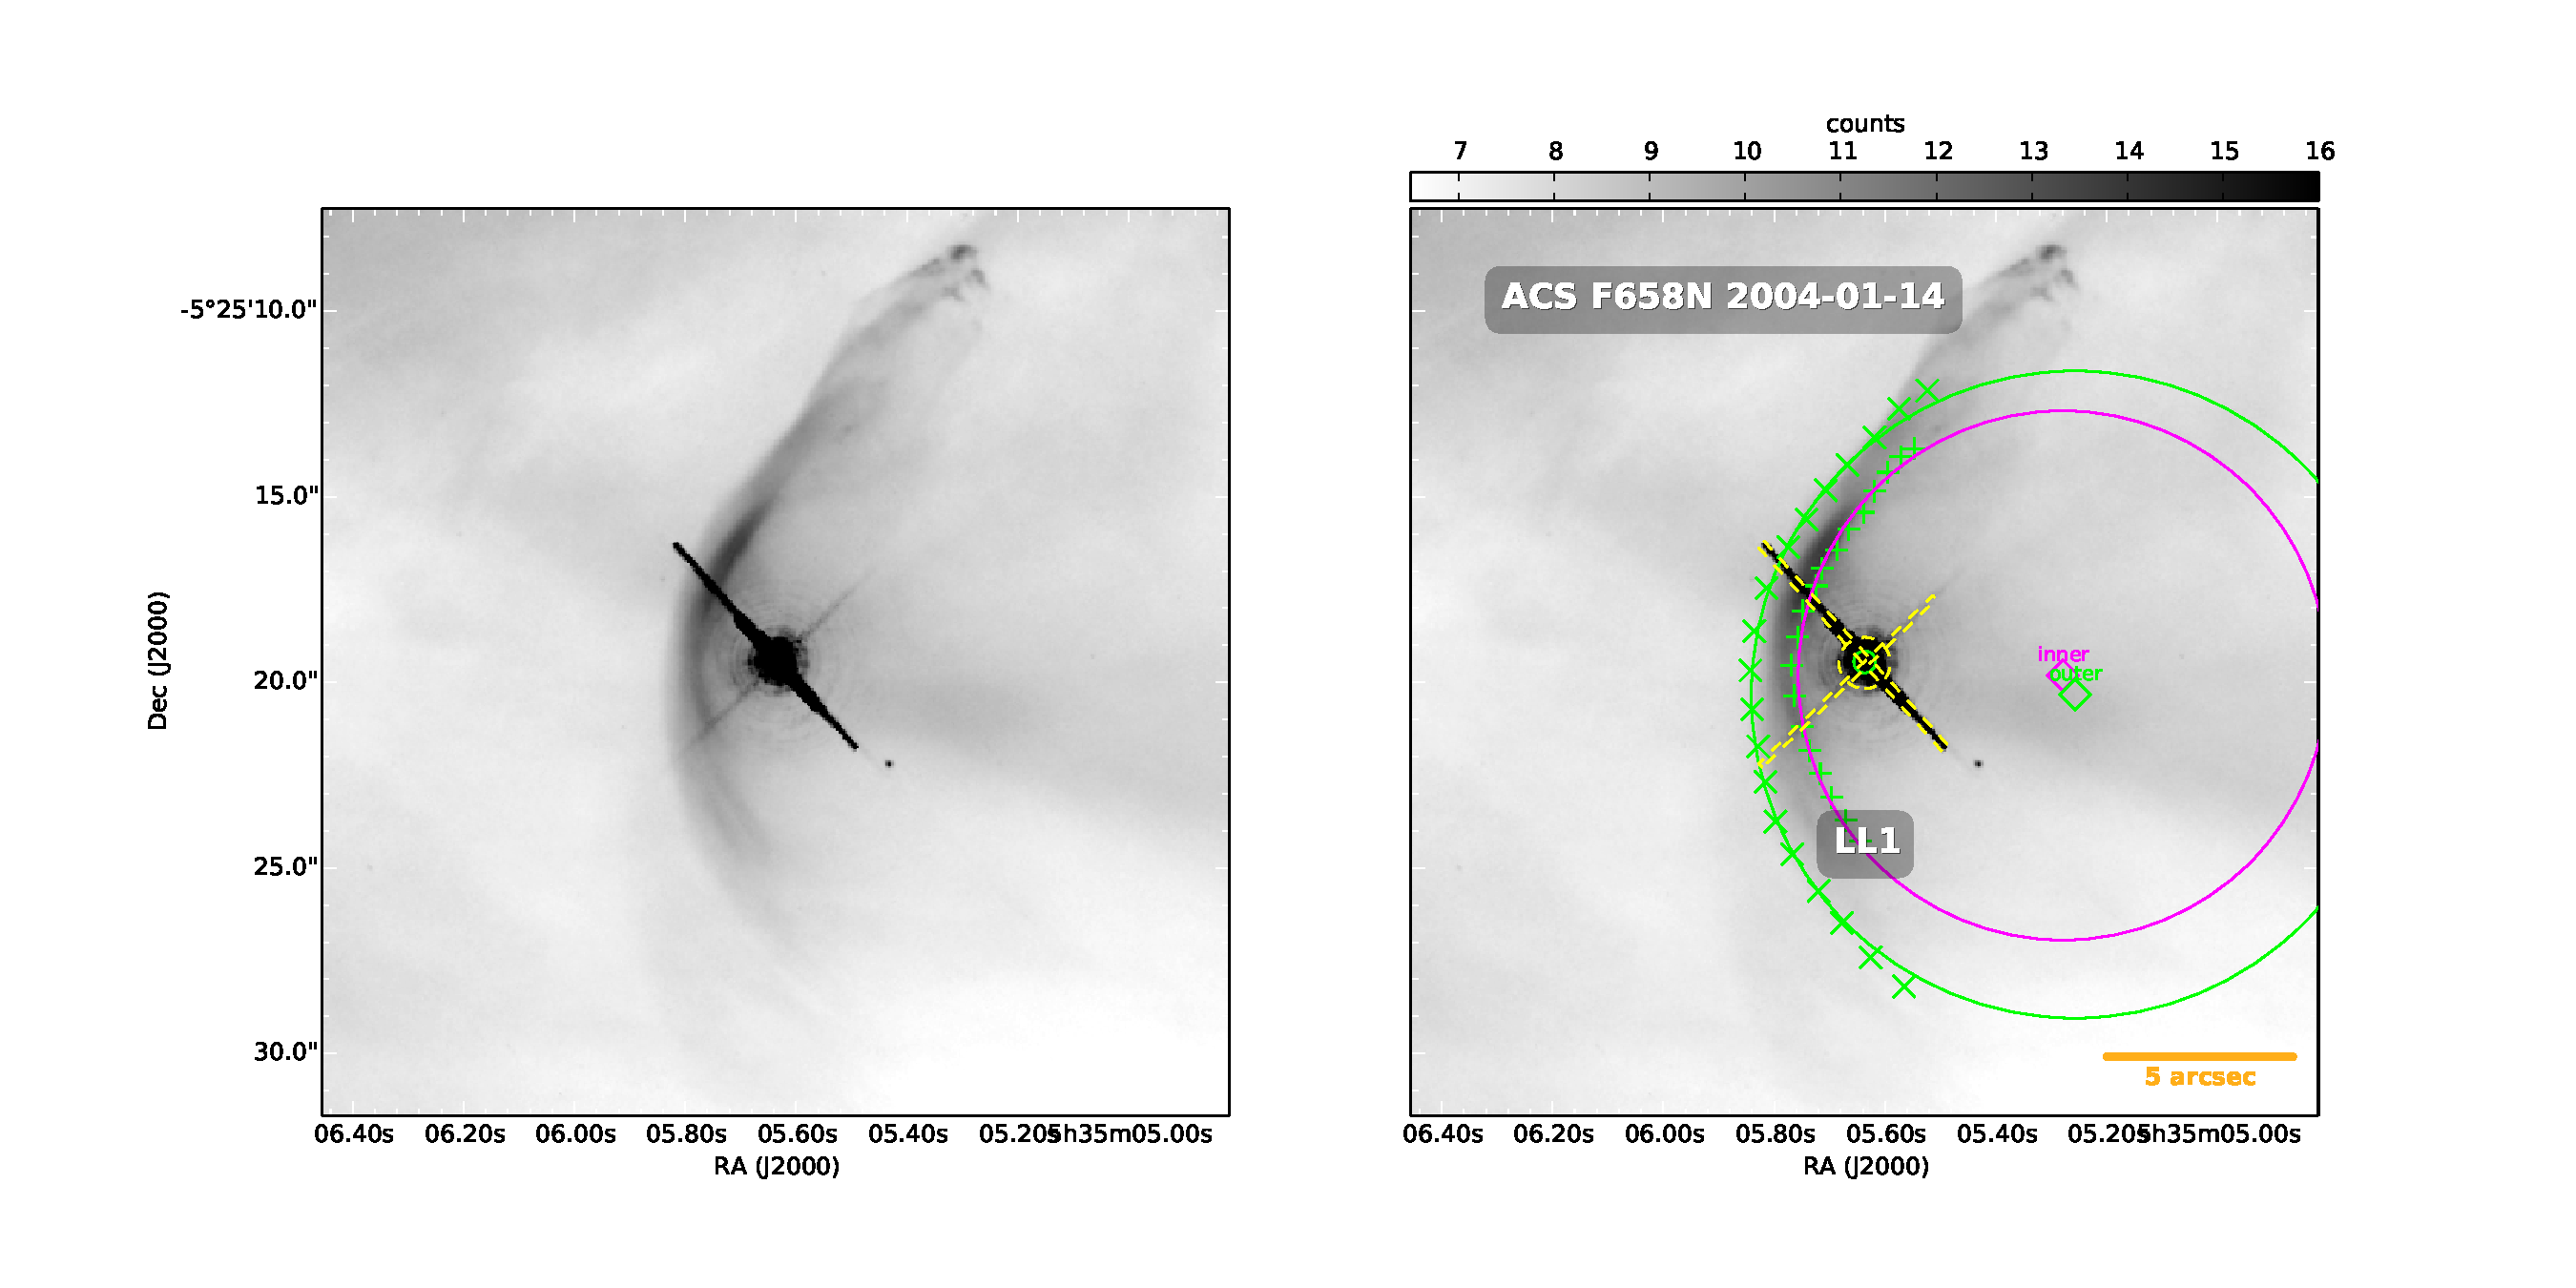
\includegraphics[width=0.5\linewidth]{./Figures/LL1-Bally_01-images} & 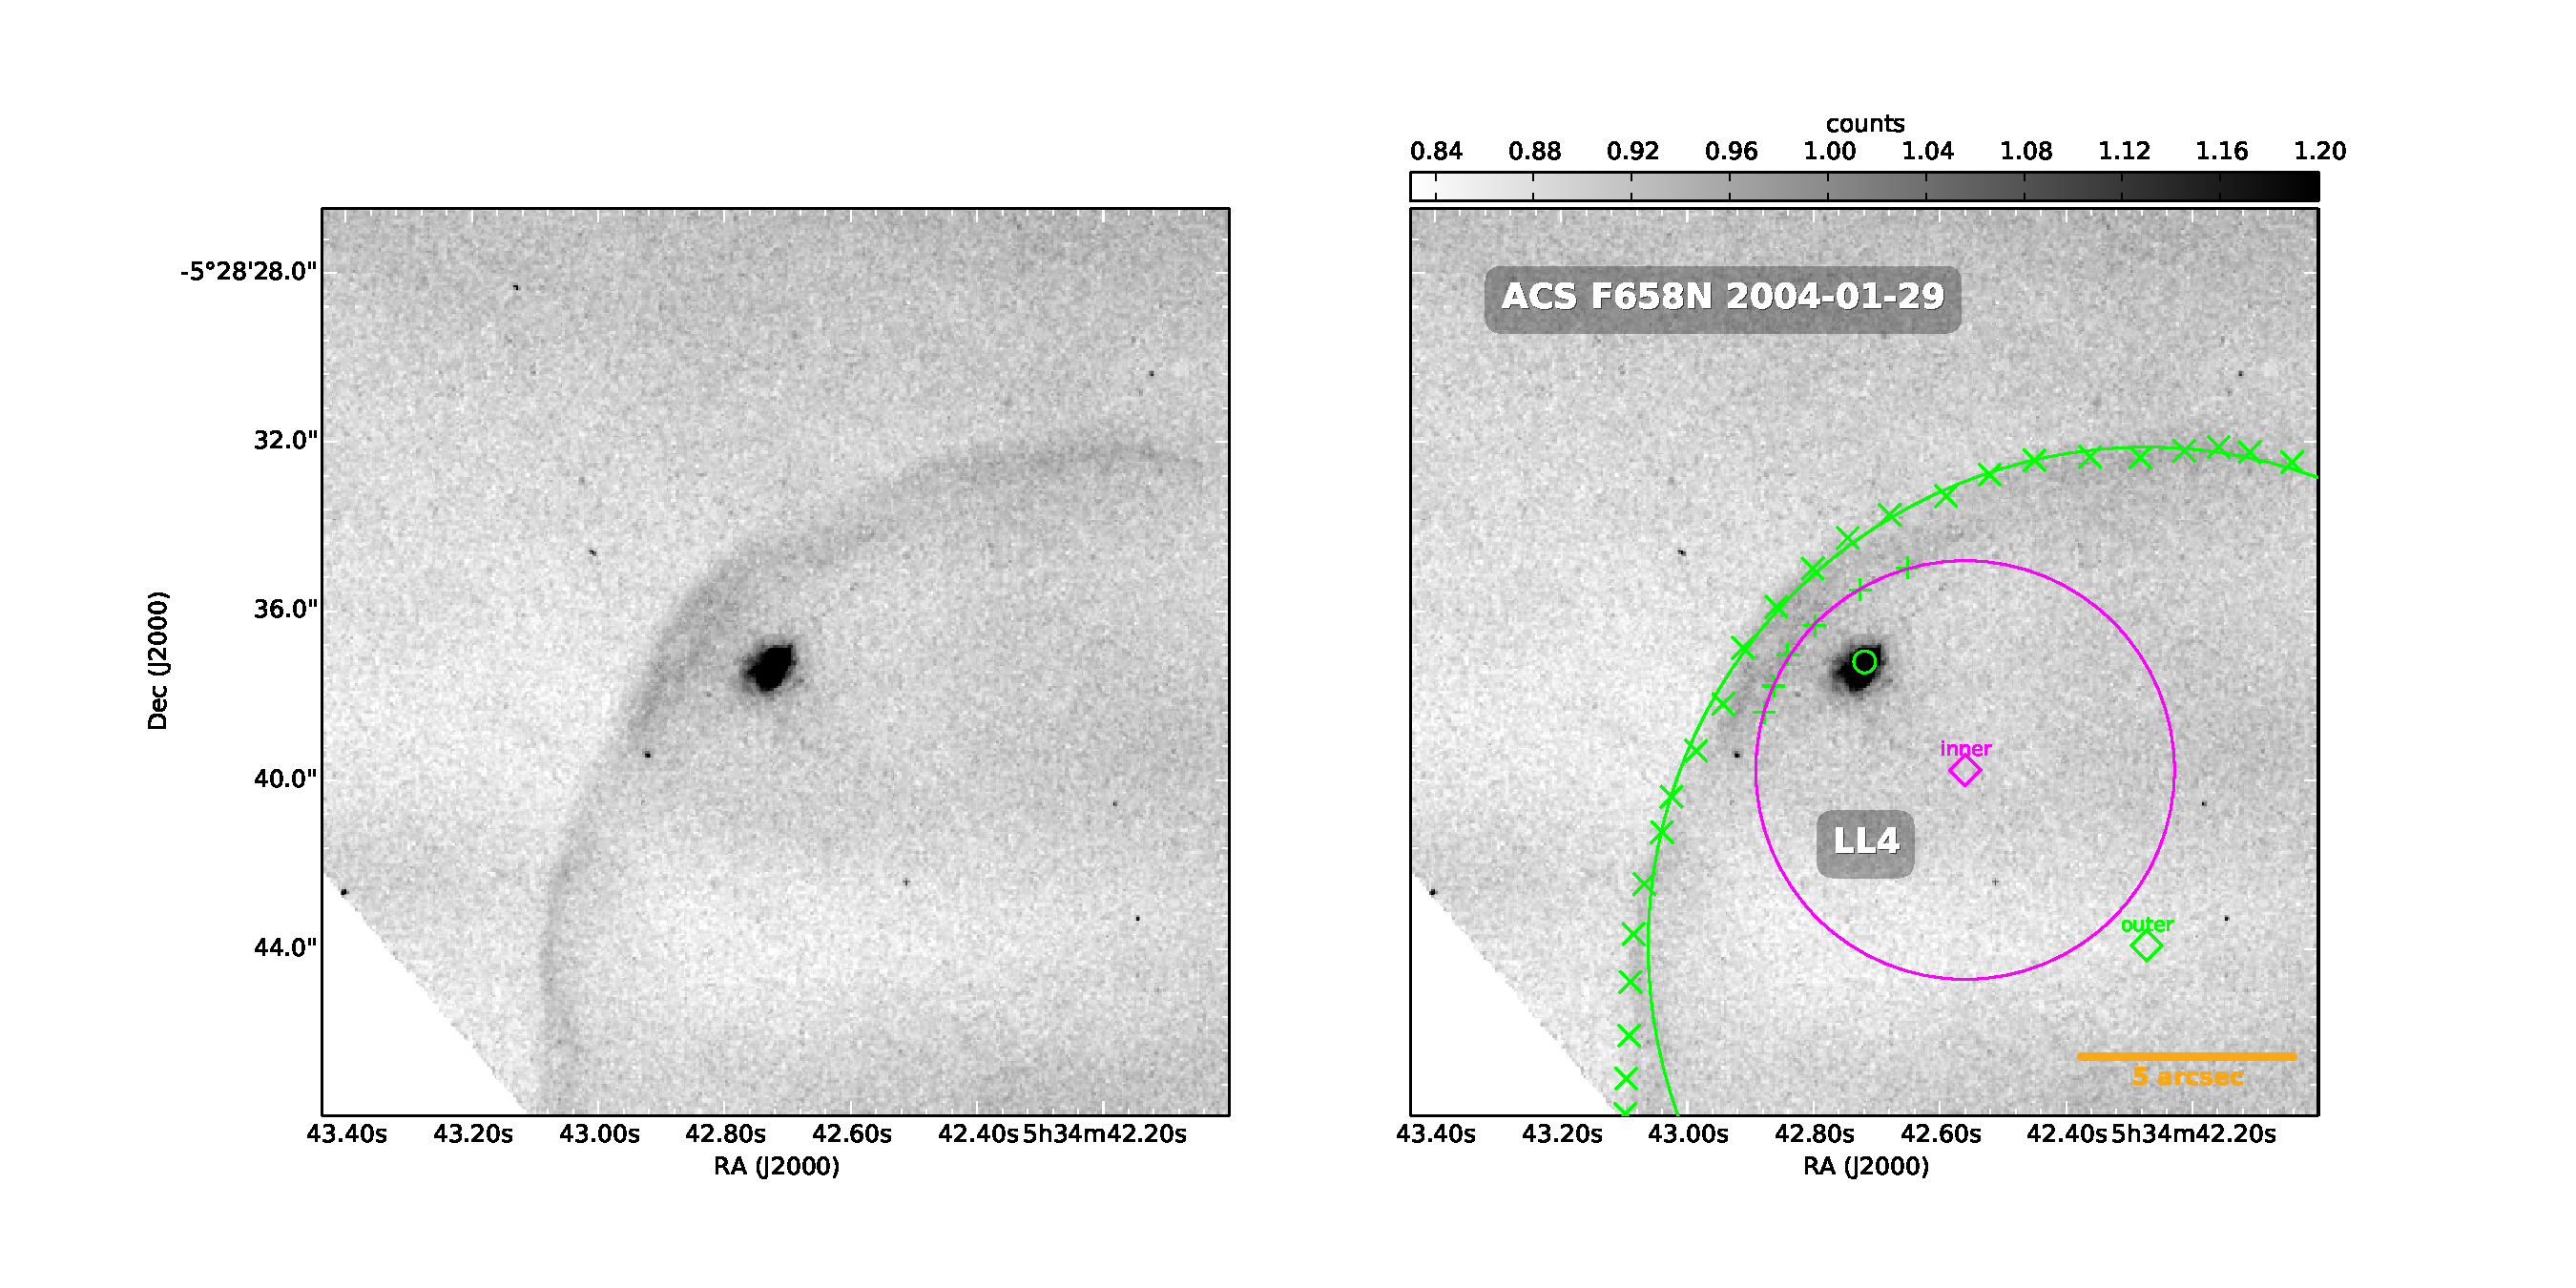
\includegraphics[width=0.5\linewidth]{./Figures/LL4-Bally_24-images} \\ 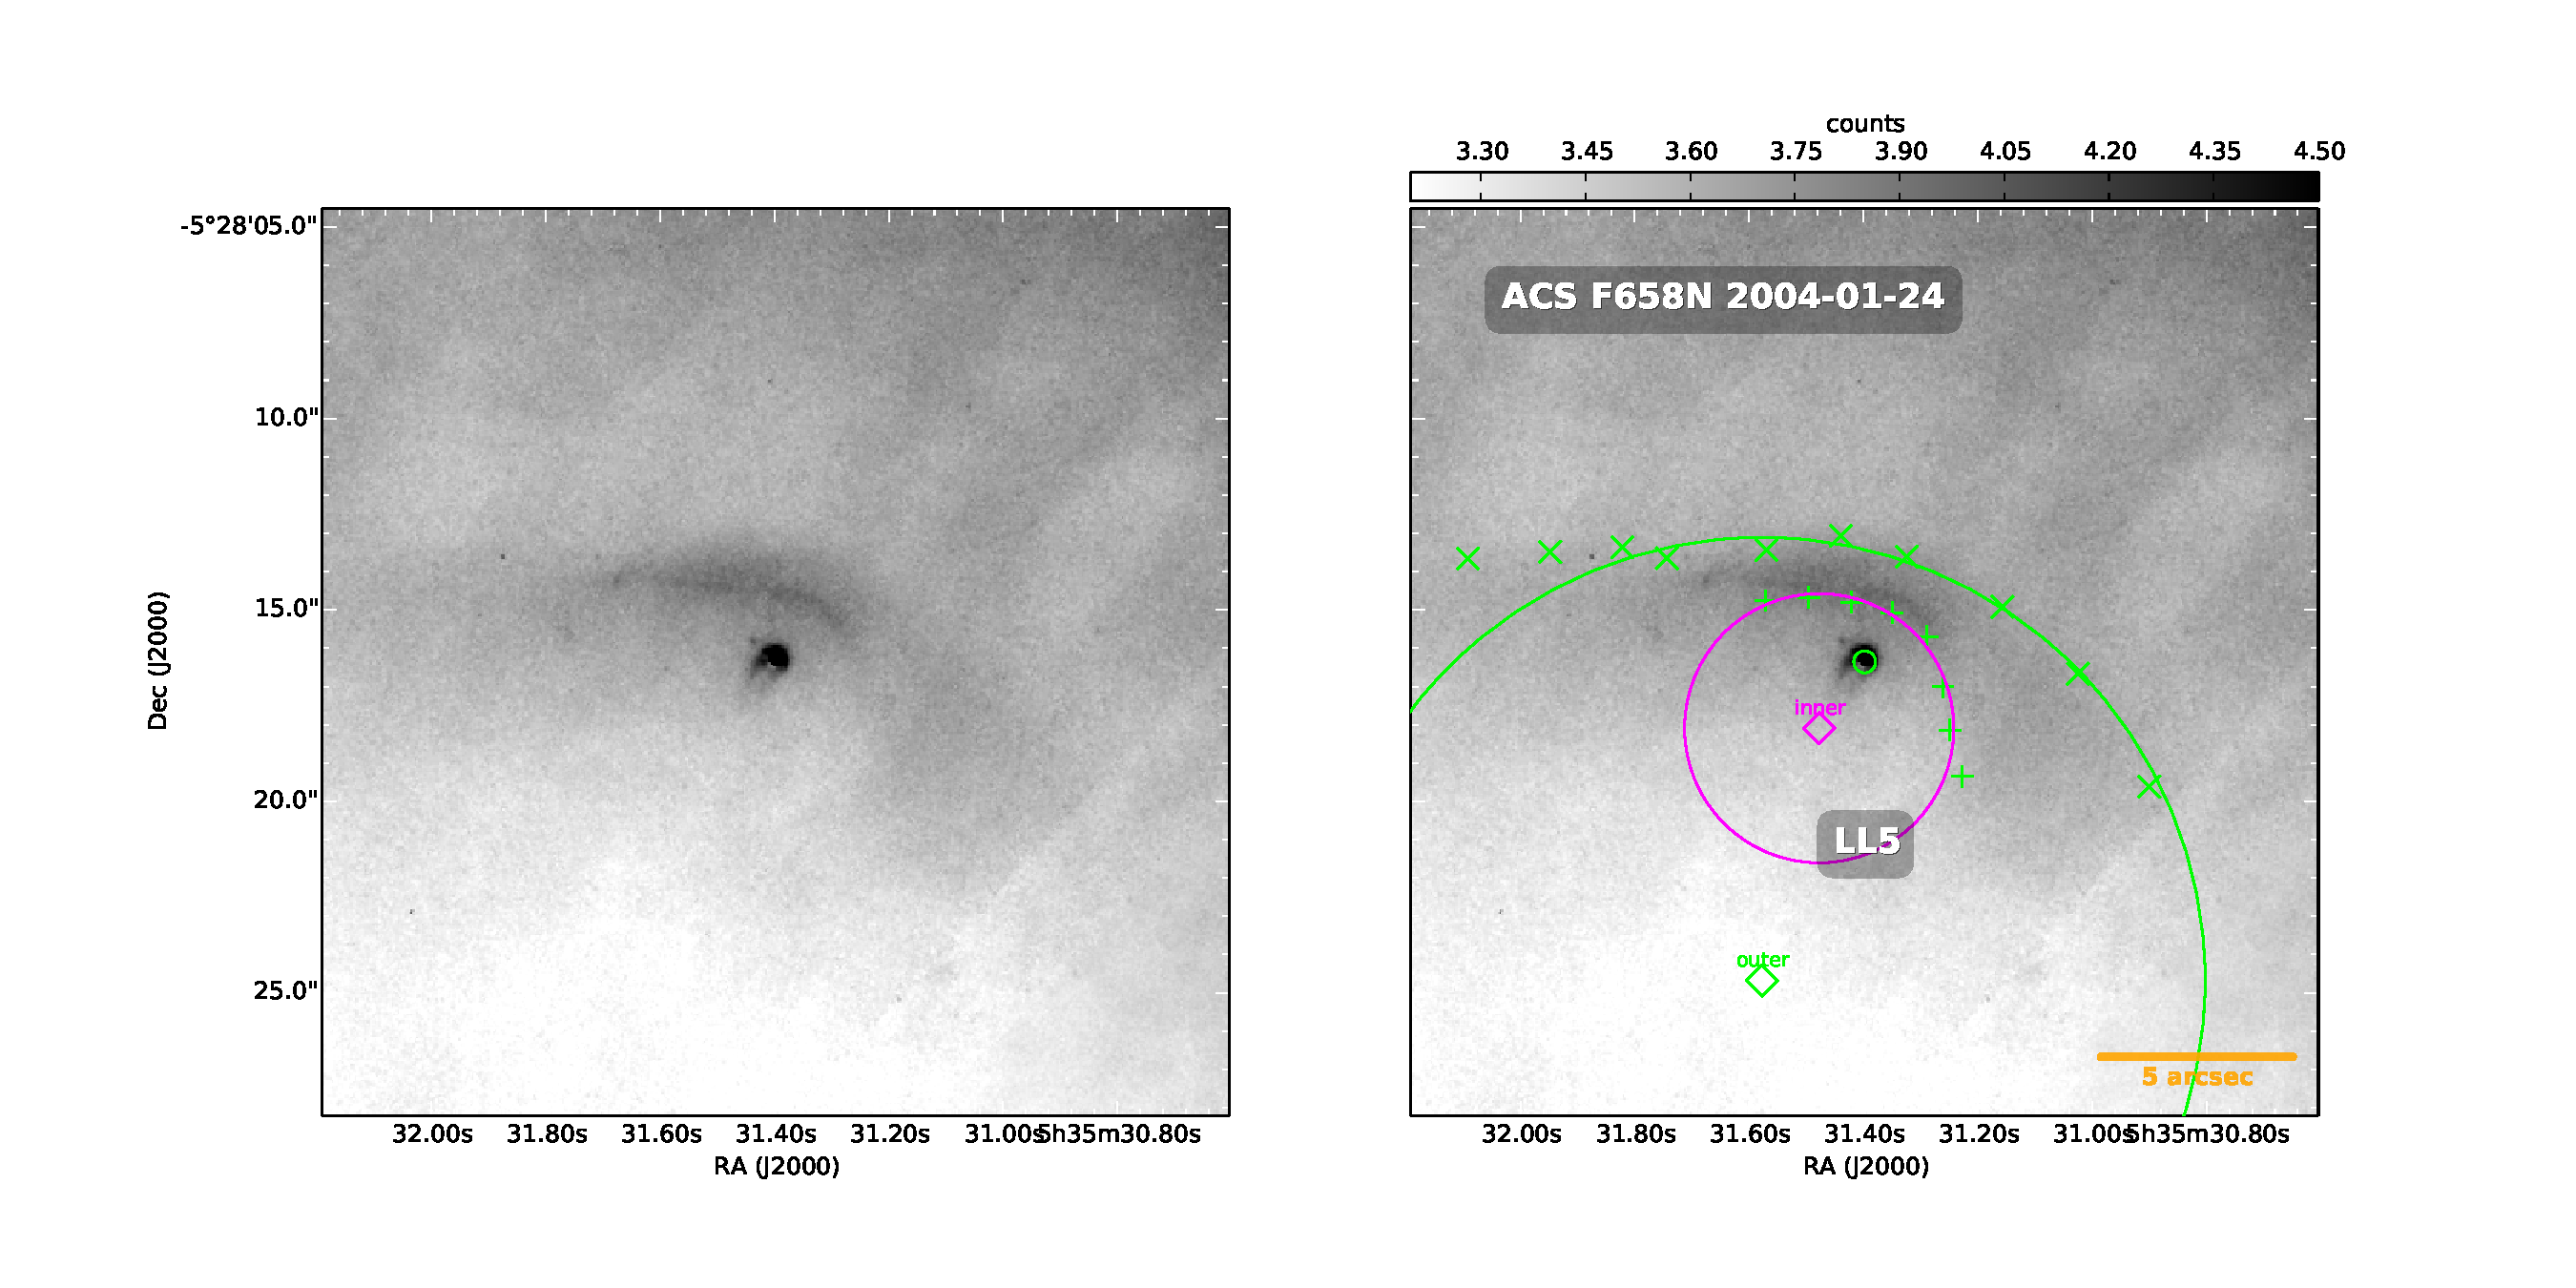
\includegraphics[width=0.5\linewidth]{./Figures/LL5-Bally_07-images} &
    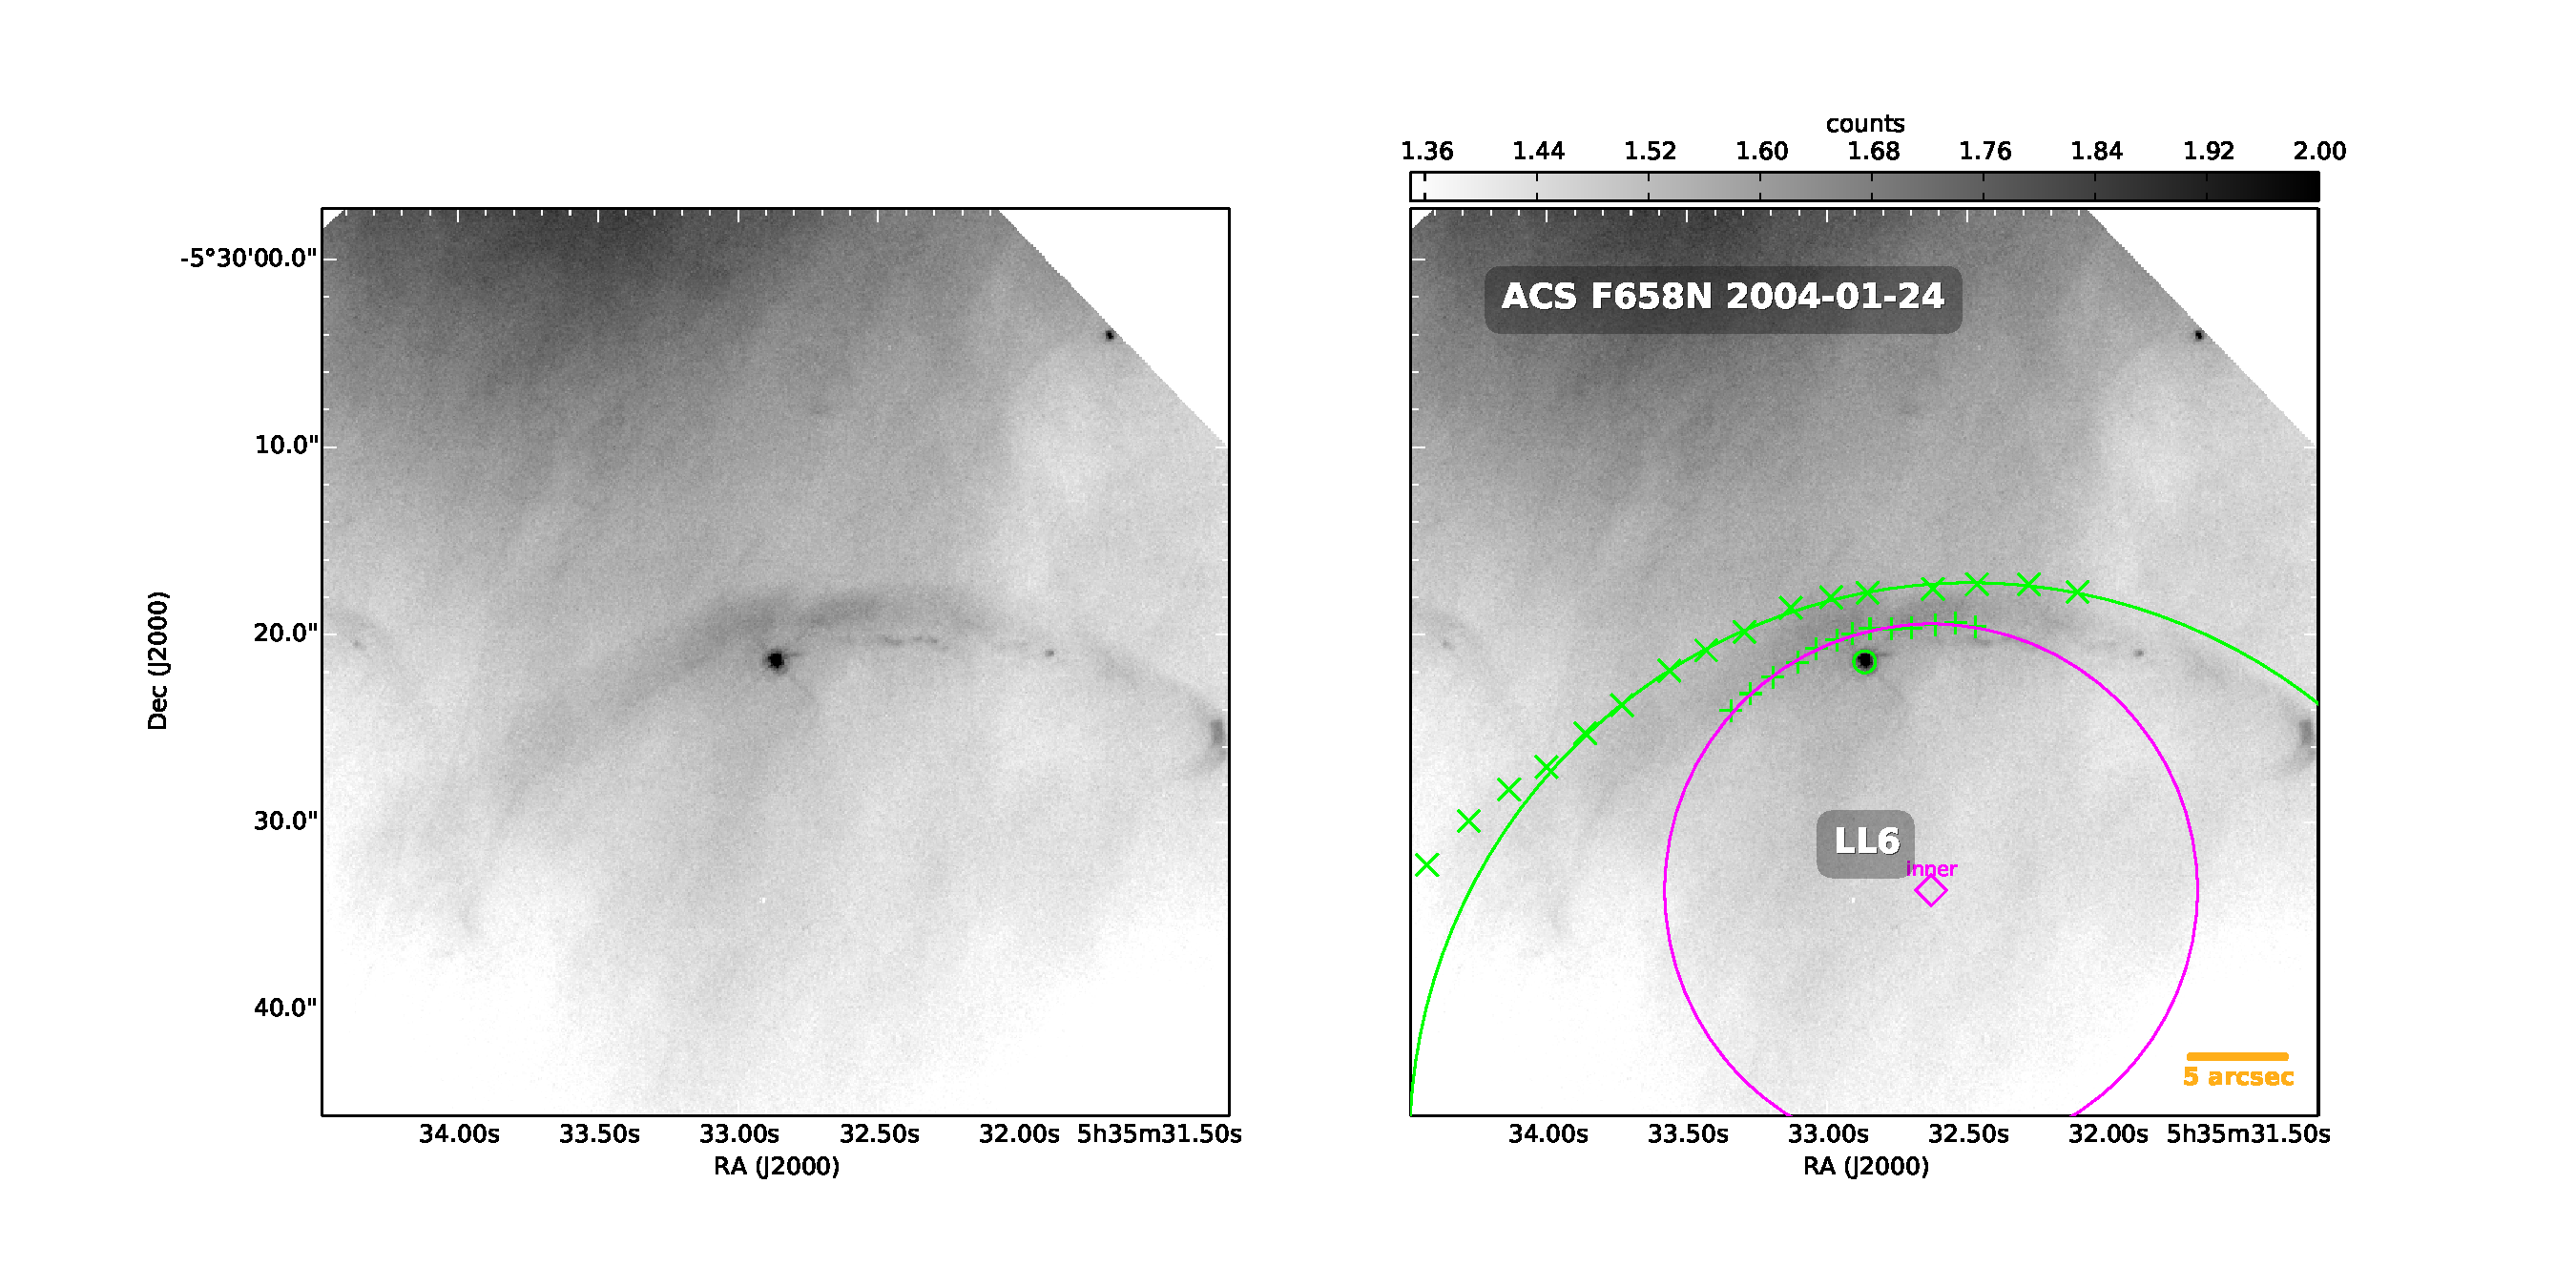
\includegraphics[width=0.5\linewidth]{./Figures/LL6-Bally_08-images} \\ 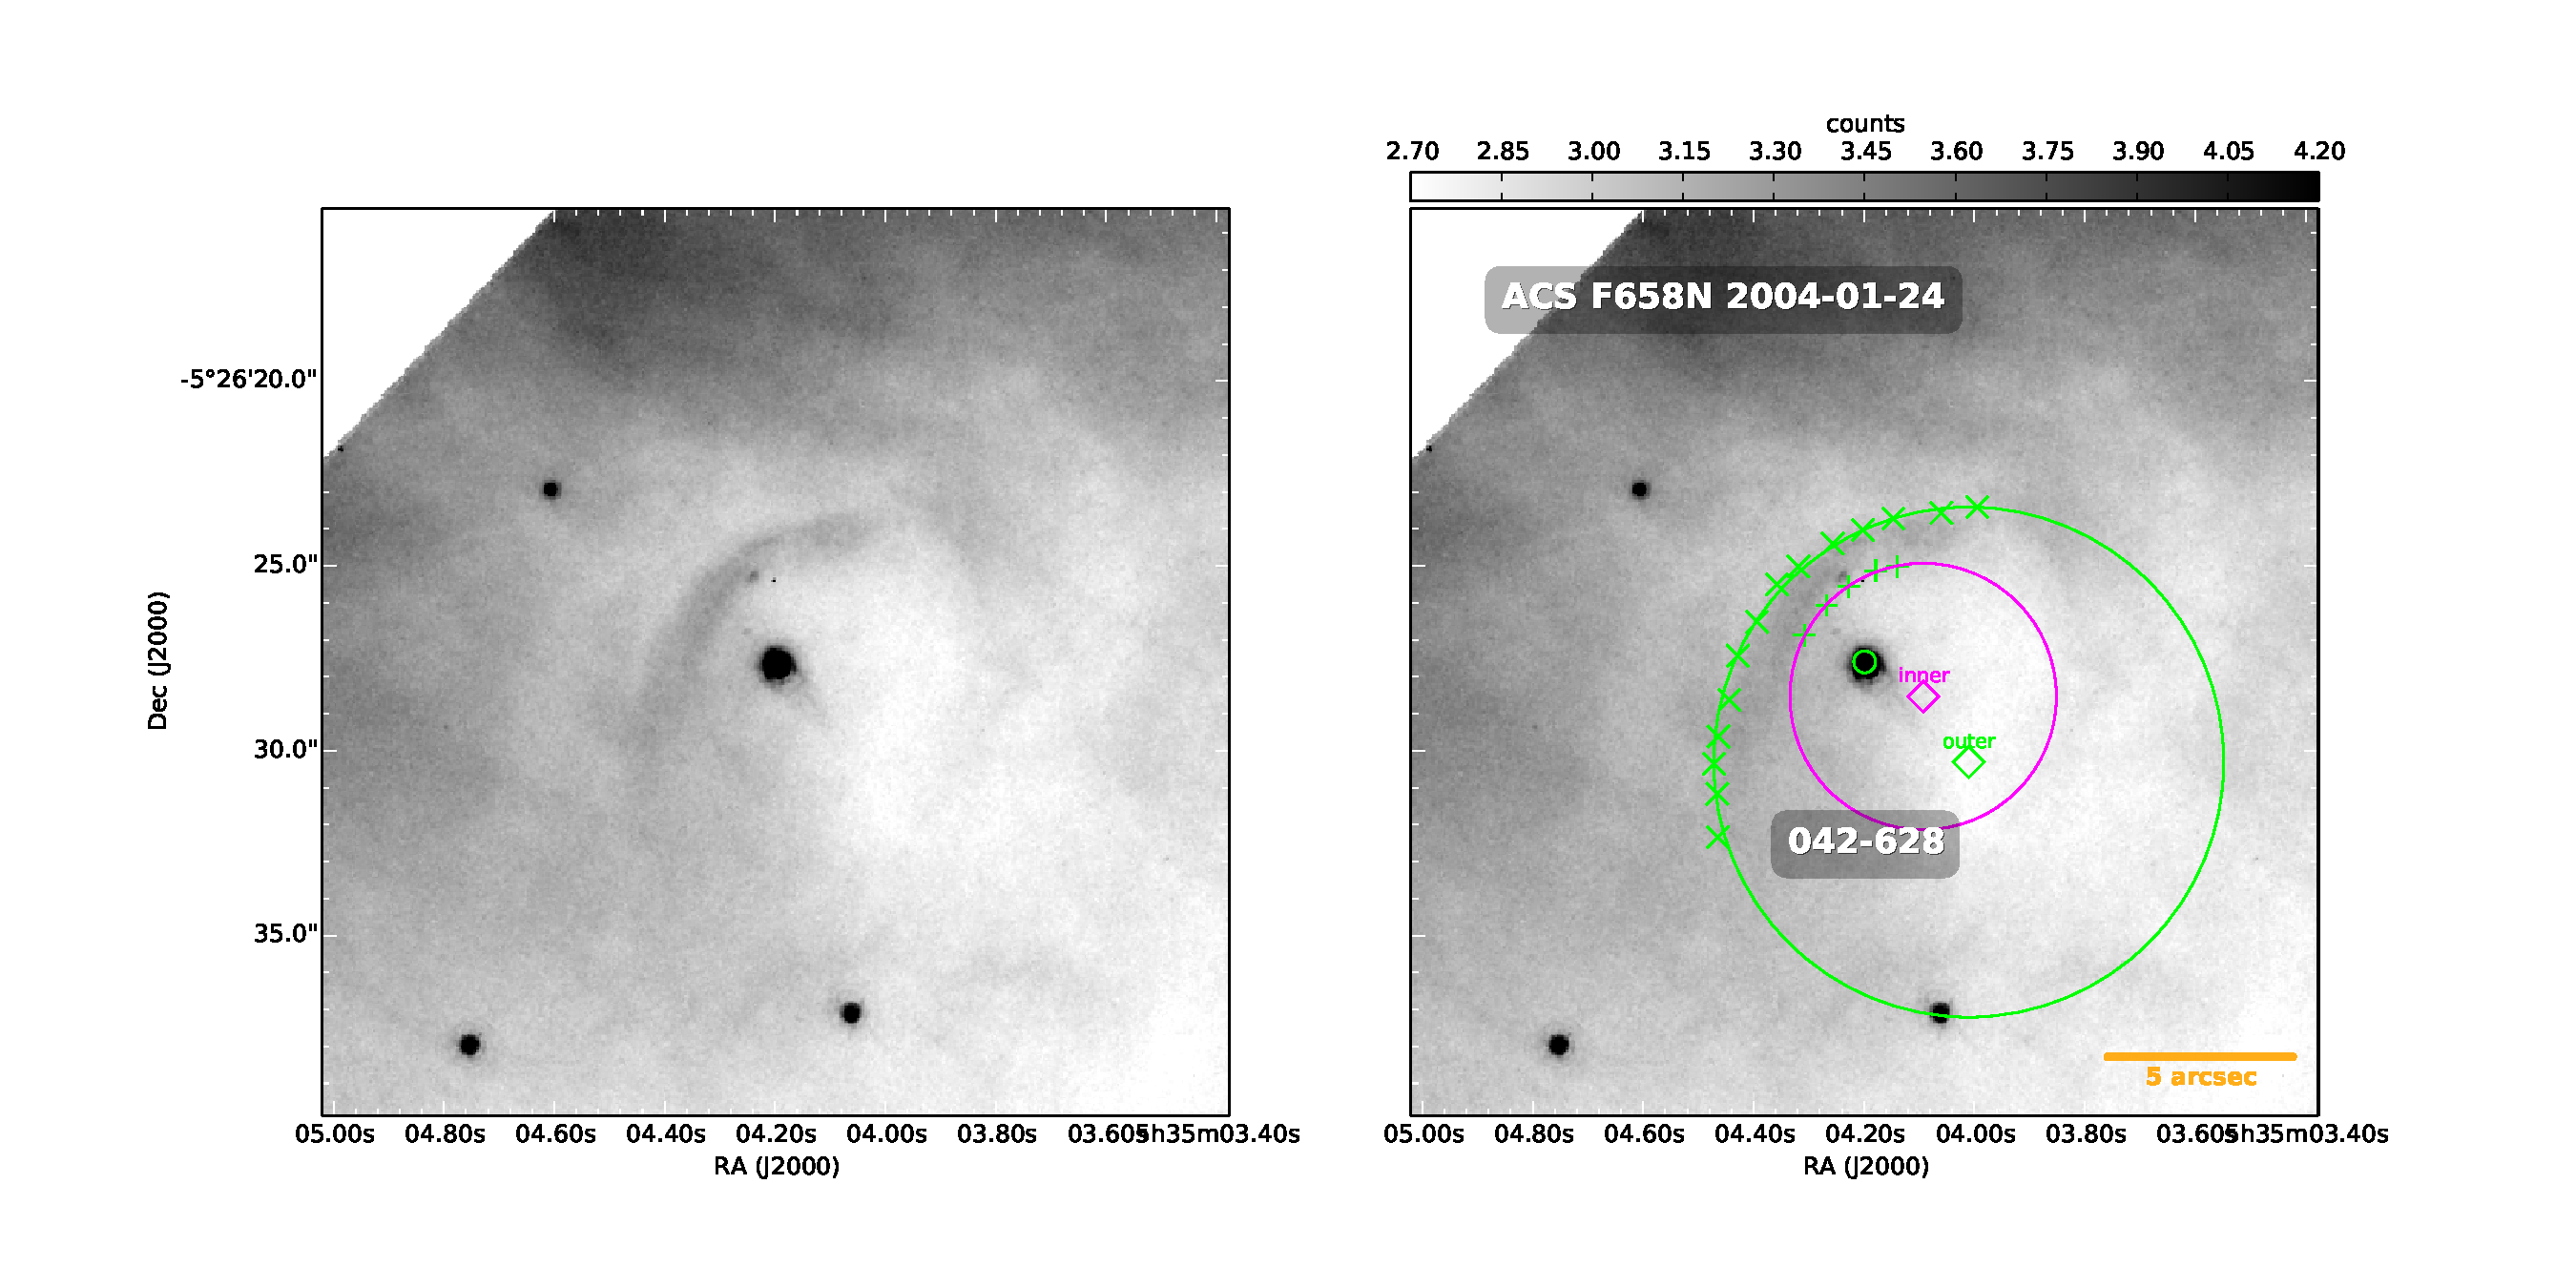
\includegraphics[width=0.5\linewidth]{./Figures/042-628-Bally_16-images} & 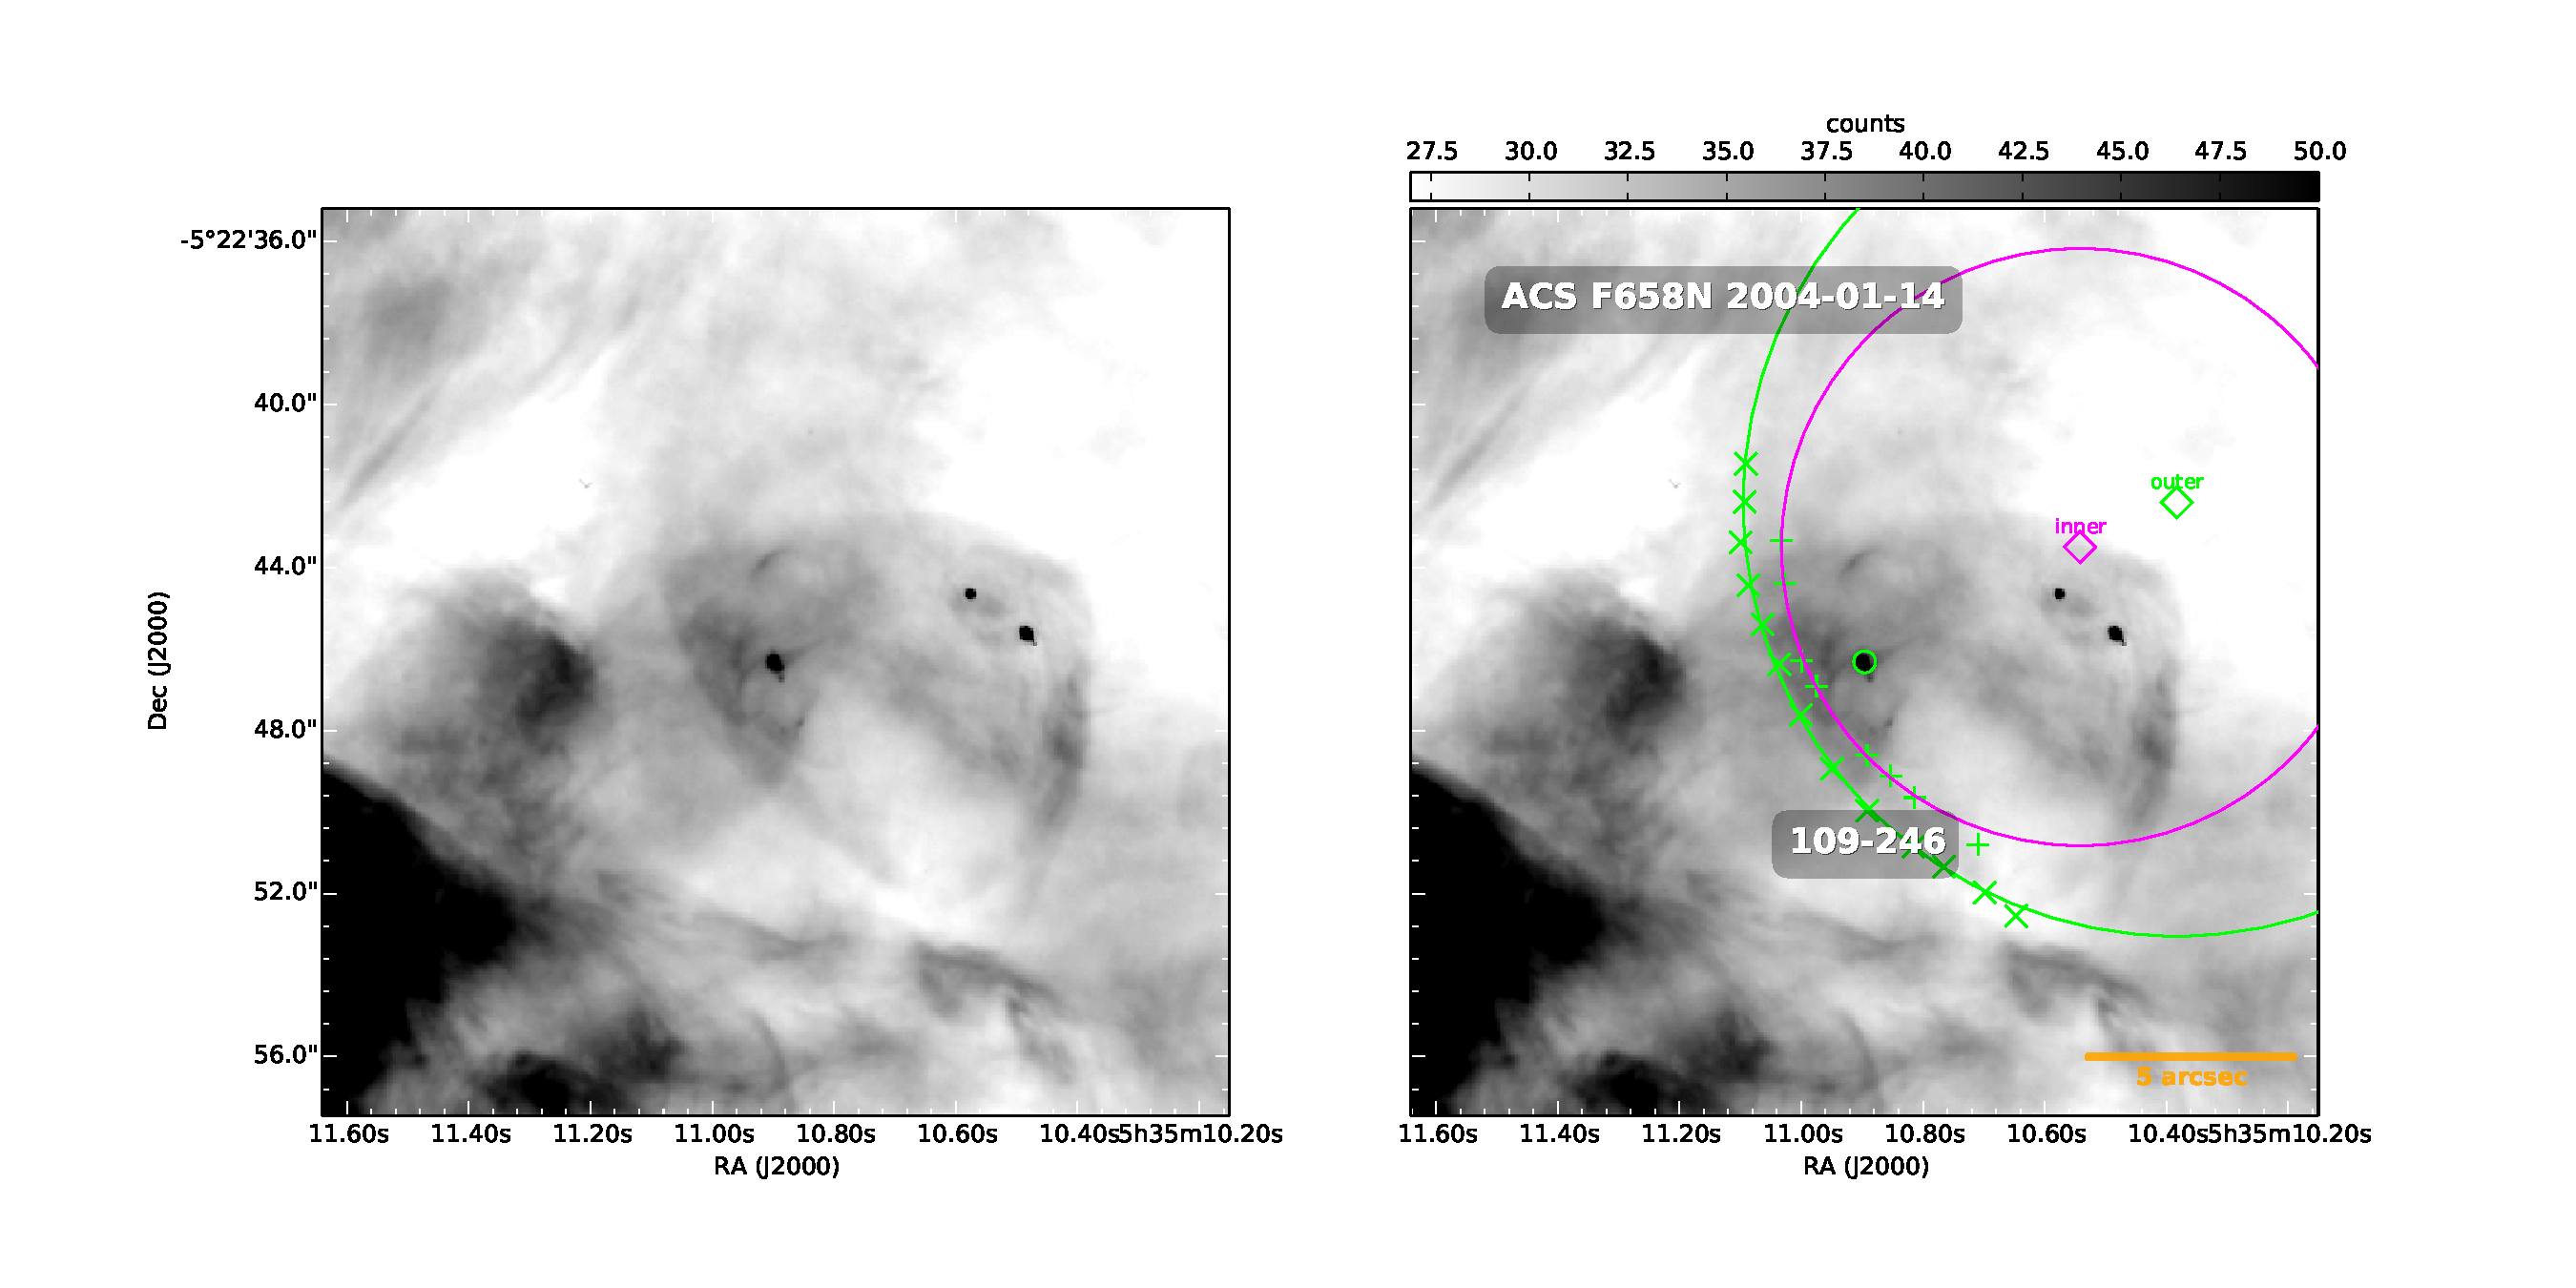
\includegraphics[width=0.5\linewidth]{./Figures/109-246-Bally_01-images} 
  \end{tabular}
  \caption{Ejemplos de objetos LL obtenidos del catálogo de \citet{Gutierrez-Soto:2015a}. A la derecha de cada panel se observa el objeto con las mediciones superpuestas de los radios característicos $(R'_0, R'_c)$ para las cáscaras exterior e interior o solo para una dependiendo del objeto. La escala de grises muestra el brillo, la barra amarilla indica la escala del objeto y las etiquetas mestran el nombre del objeto, el instrumento que se utilizó para obtener la imagen y la fecha en que se obtuvo.}
  \label{fig:Luis-mosaic-1}
\end{figure}


\begin{figure}
  \ContinuedFloat
    \captionsetup{list=off,format=cont}
  \begin{tabular}{cc}
    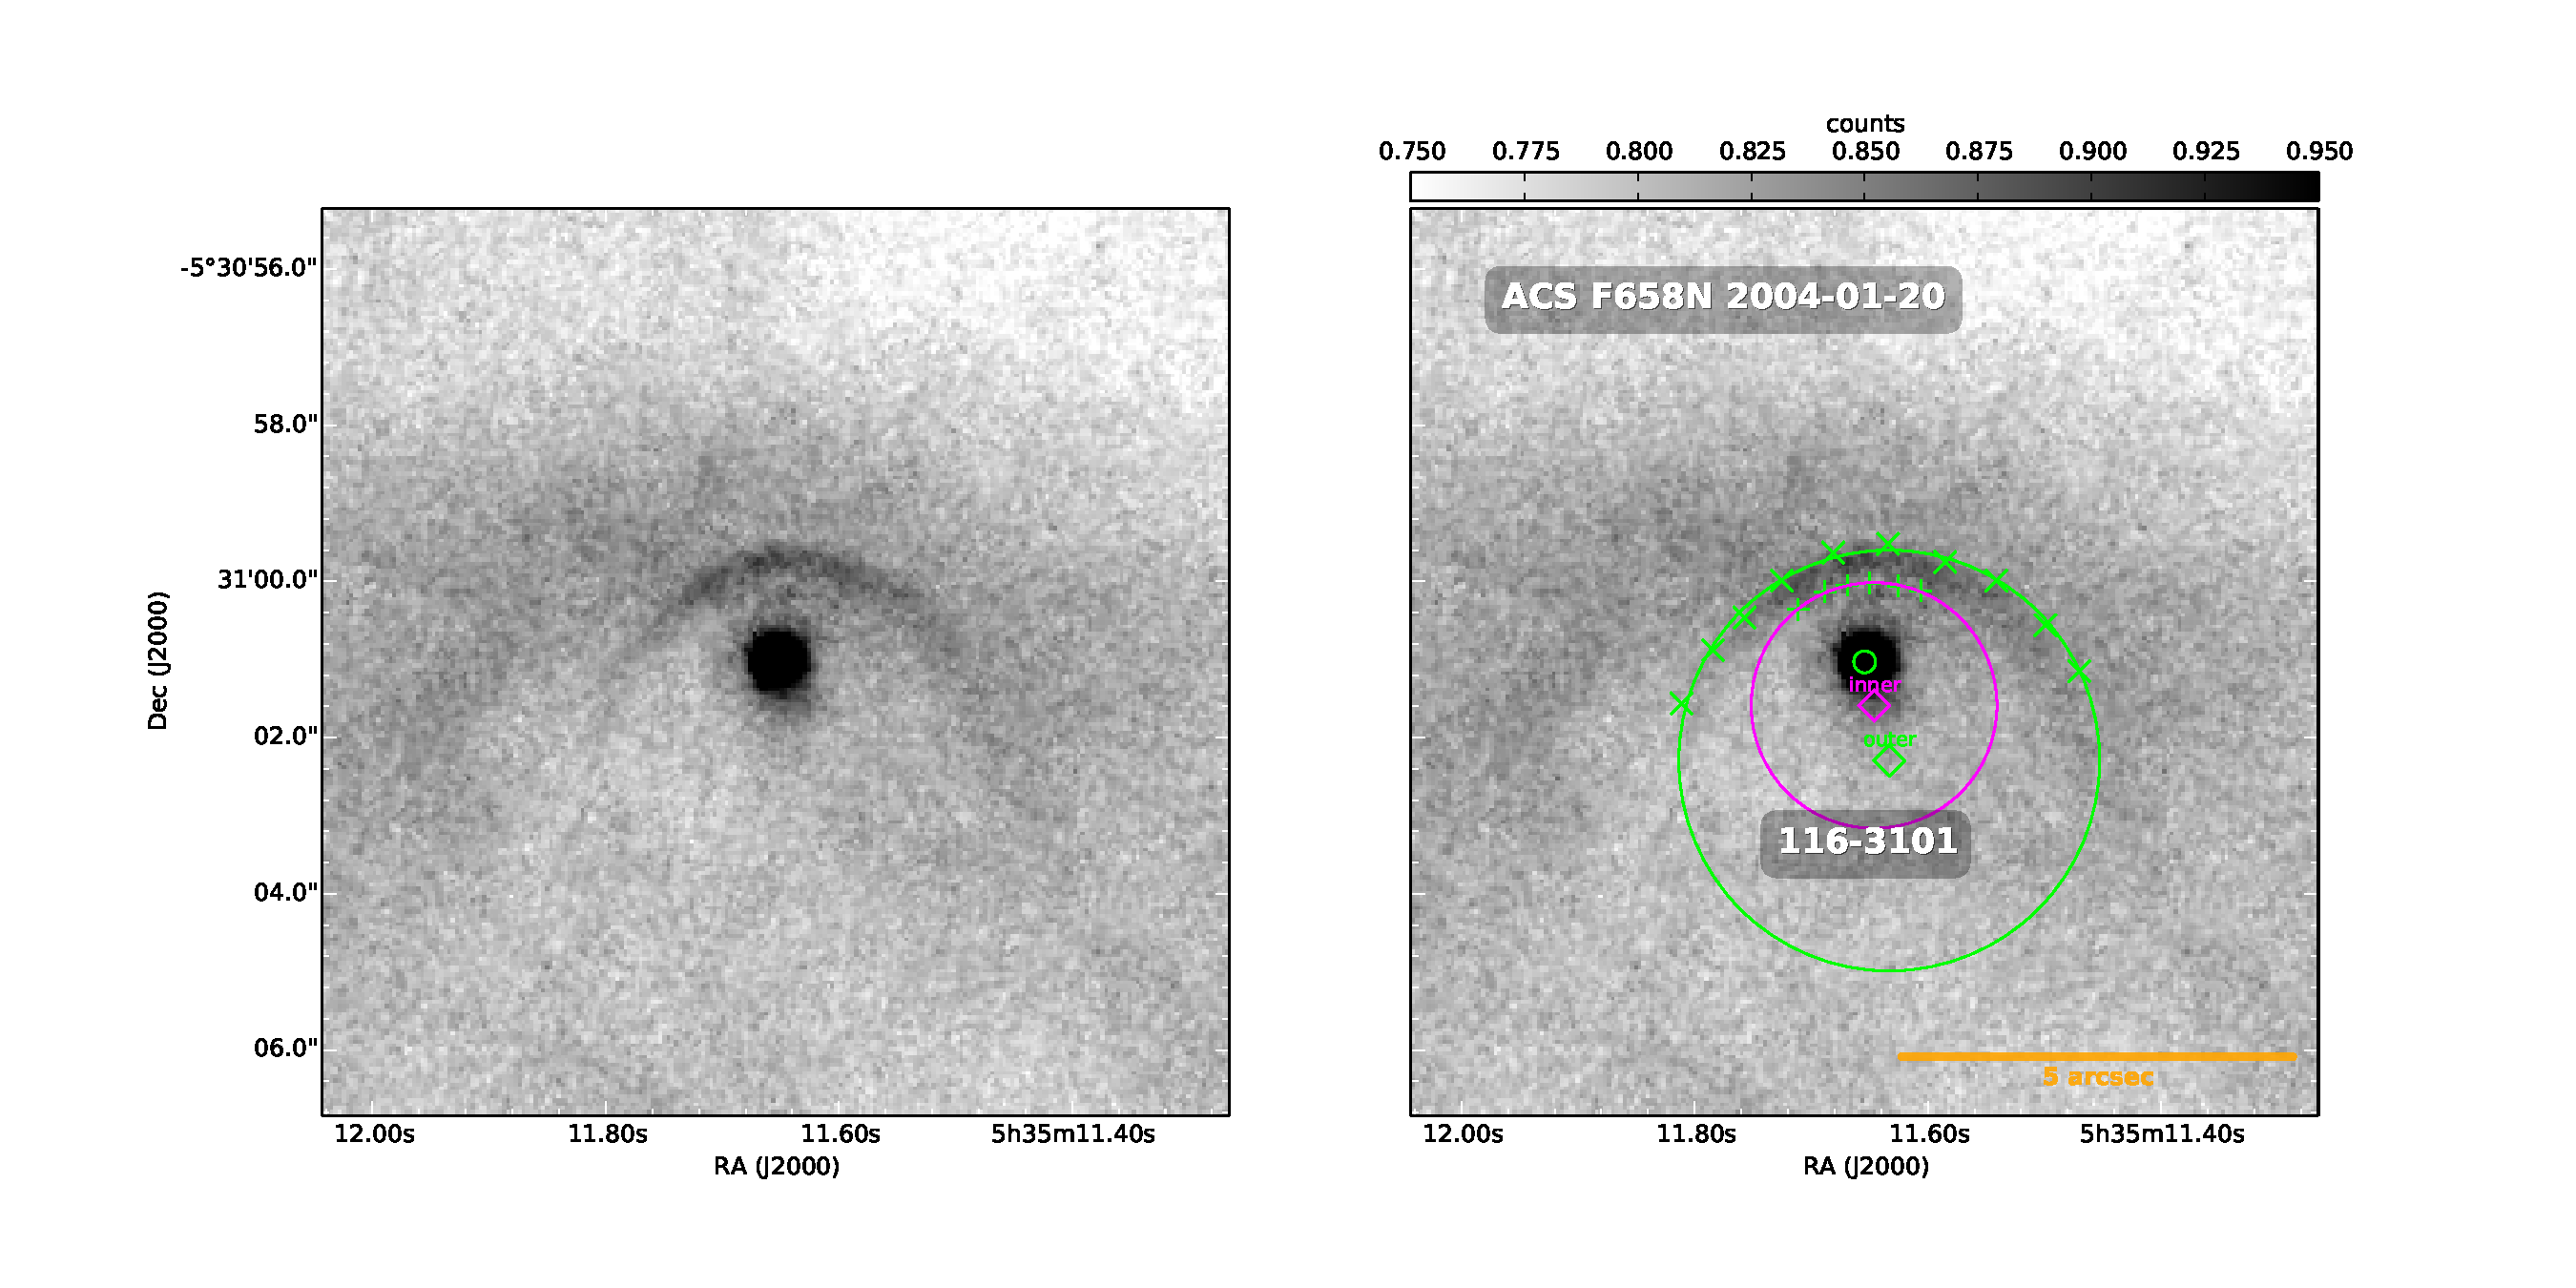
\includegraphics[width=0.5\linewidth]{./Figures/116-3101-Bally_14-images} & 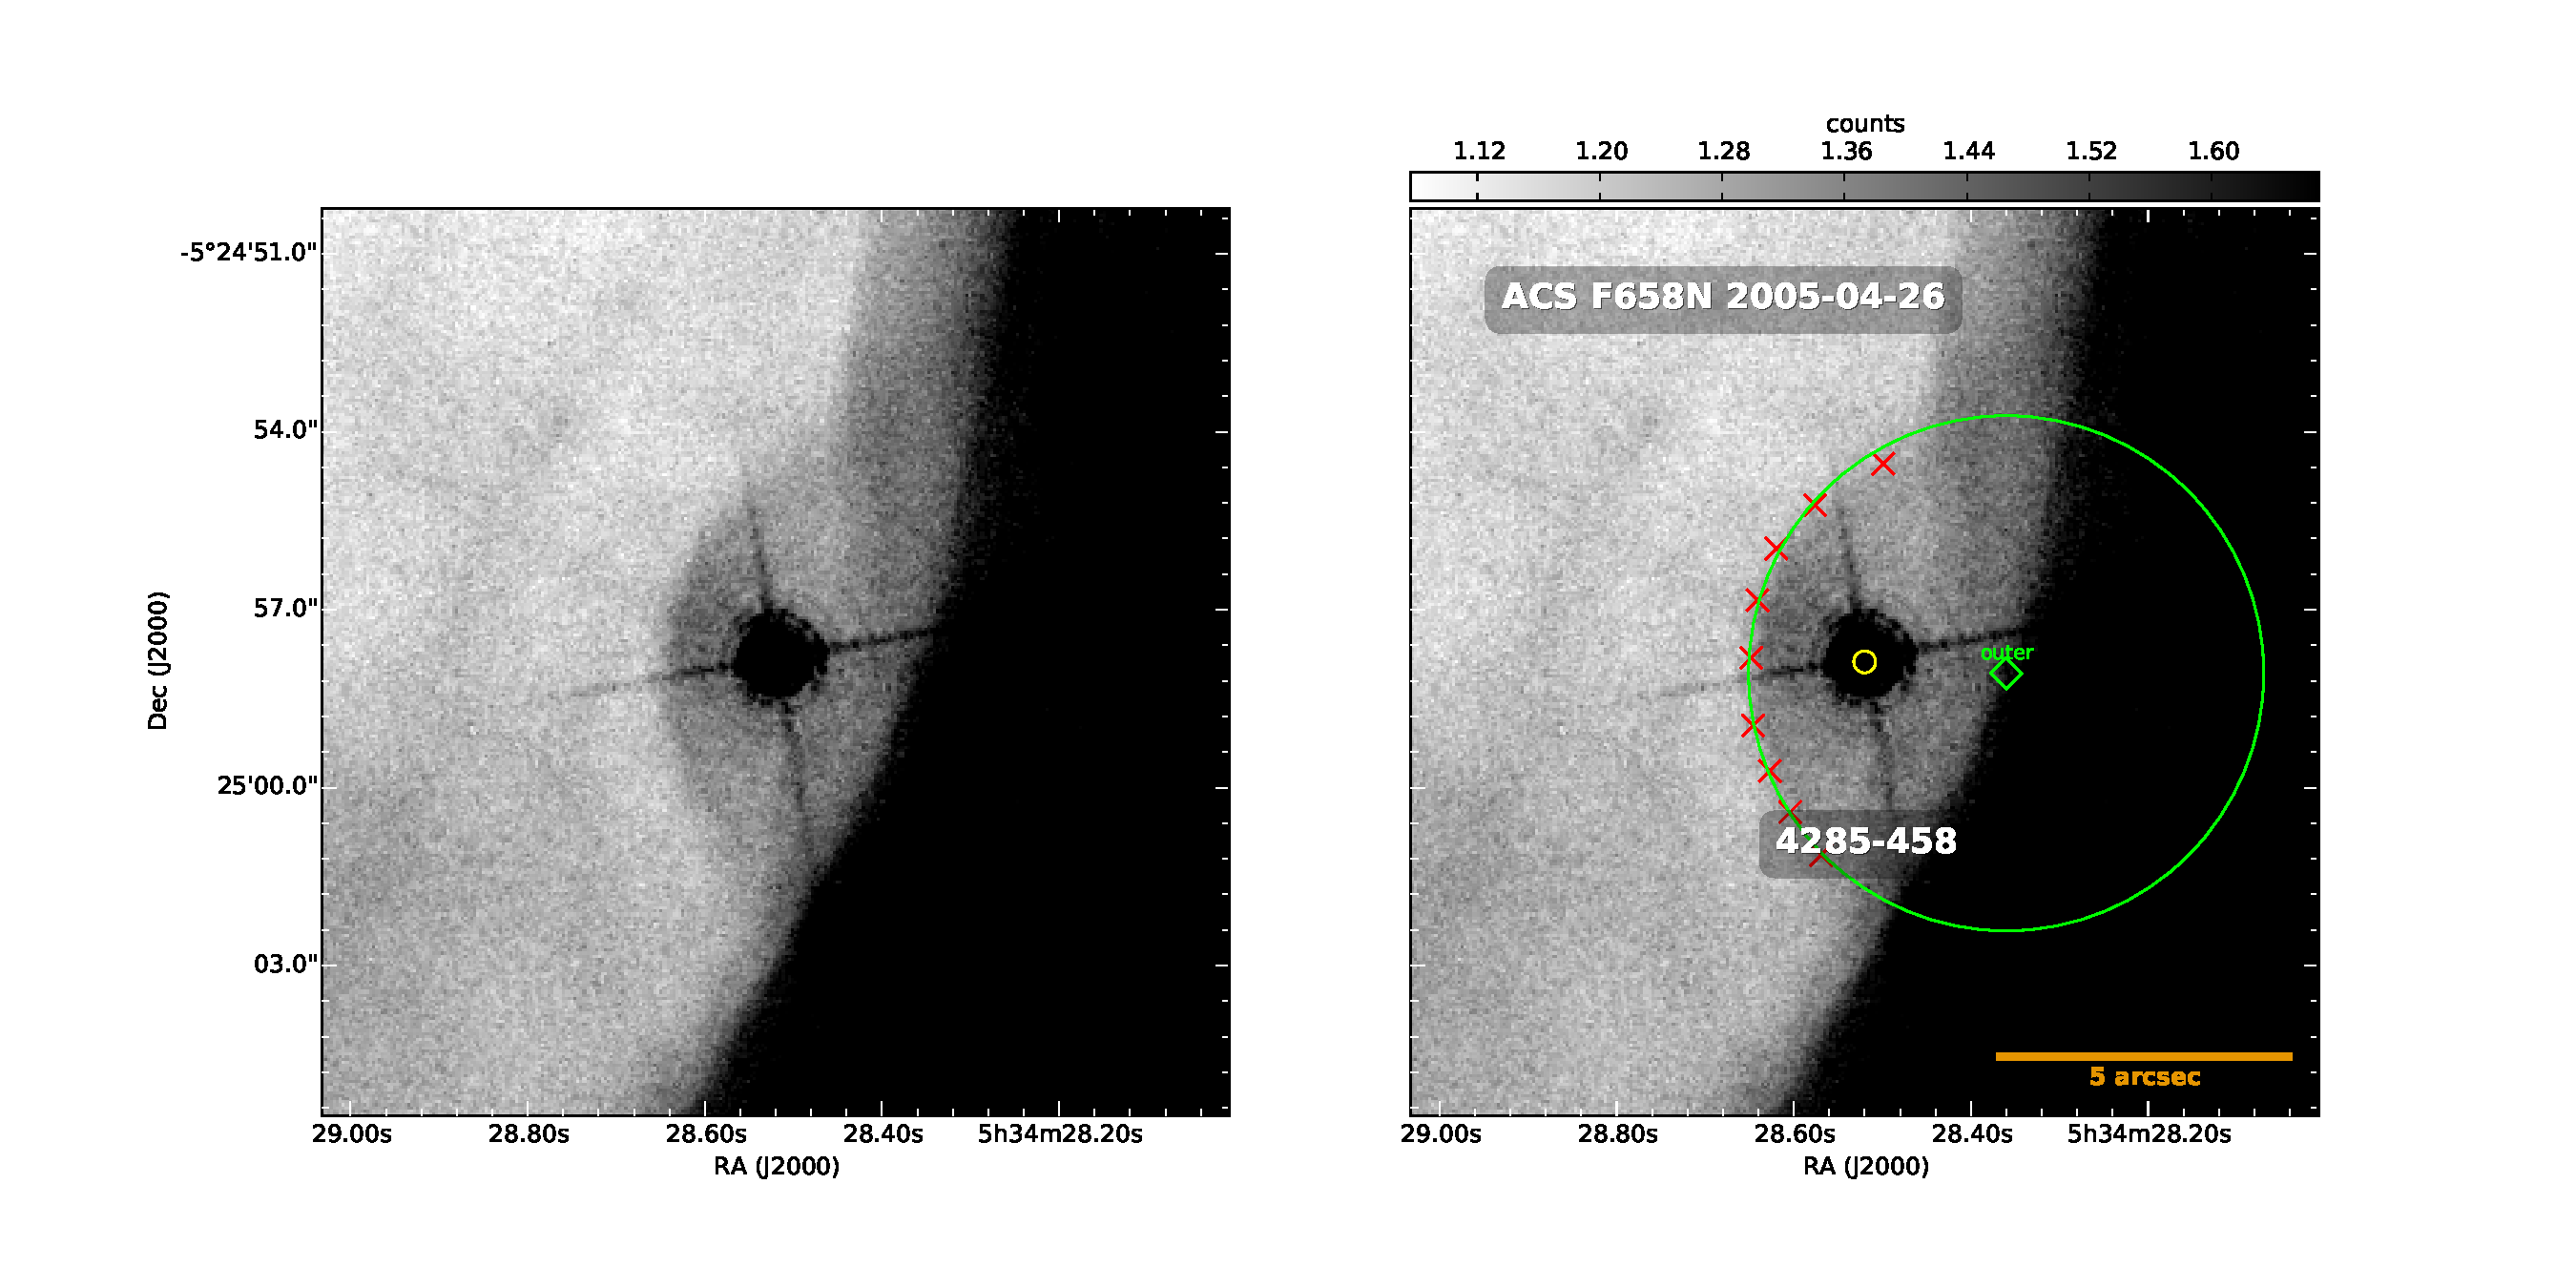
\includegraphics[width=0.5\linewidth]{./Figures/4285-458-Robberto_ACS_1r_f658n-images} \\ 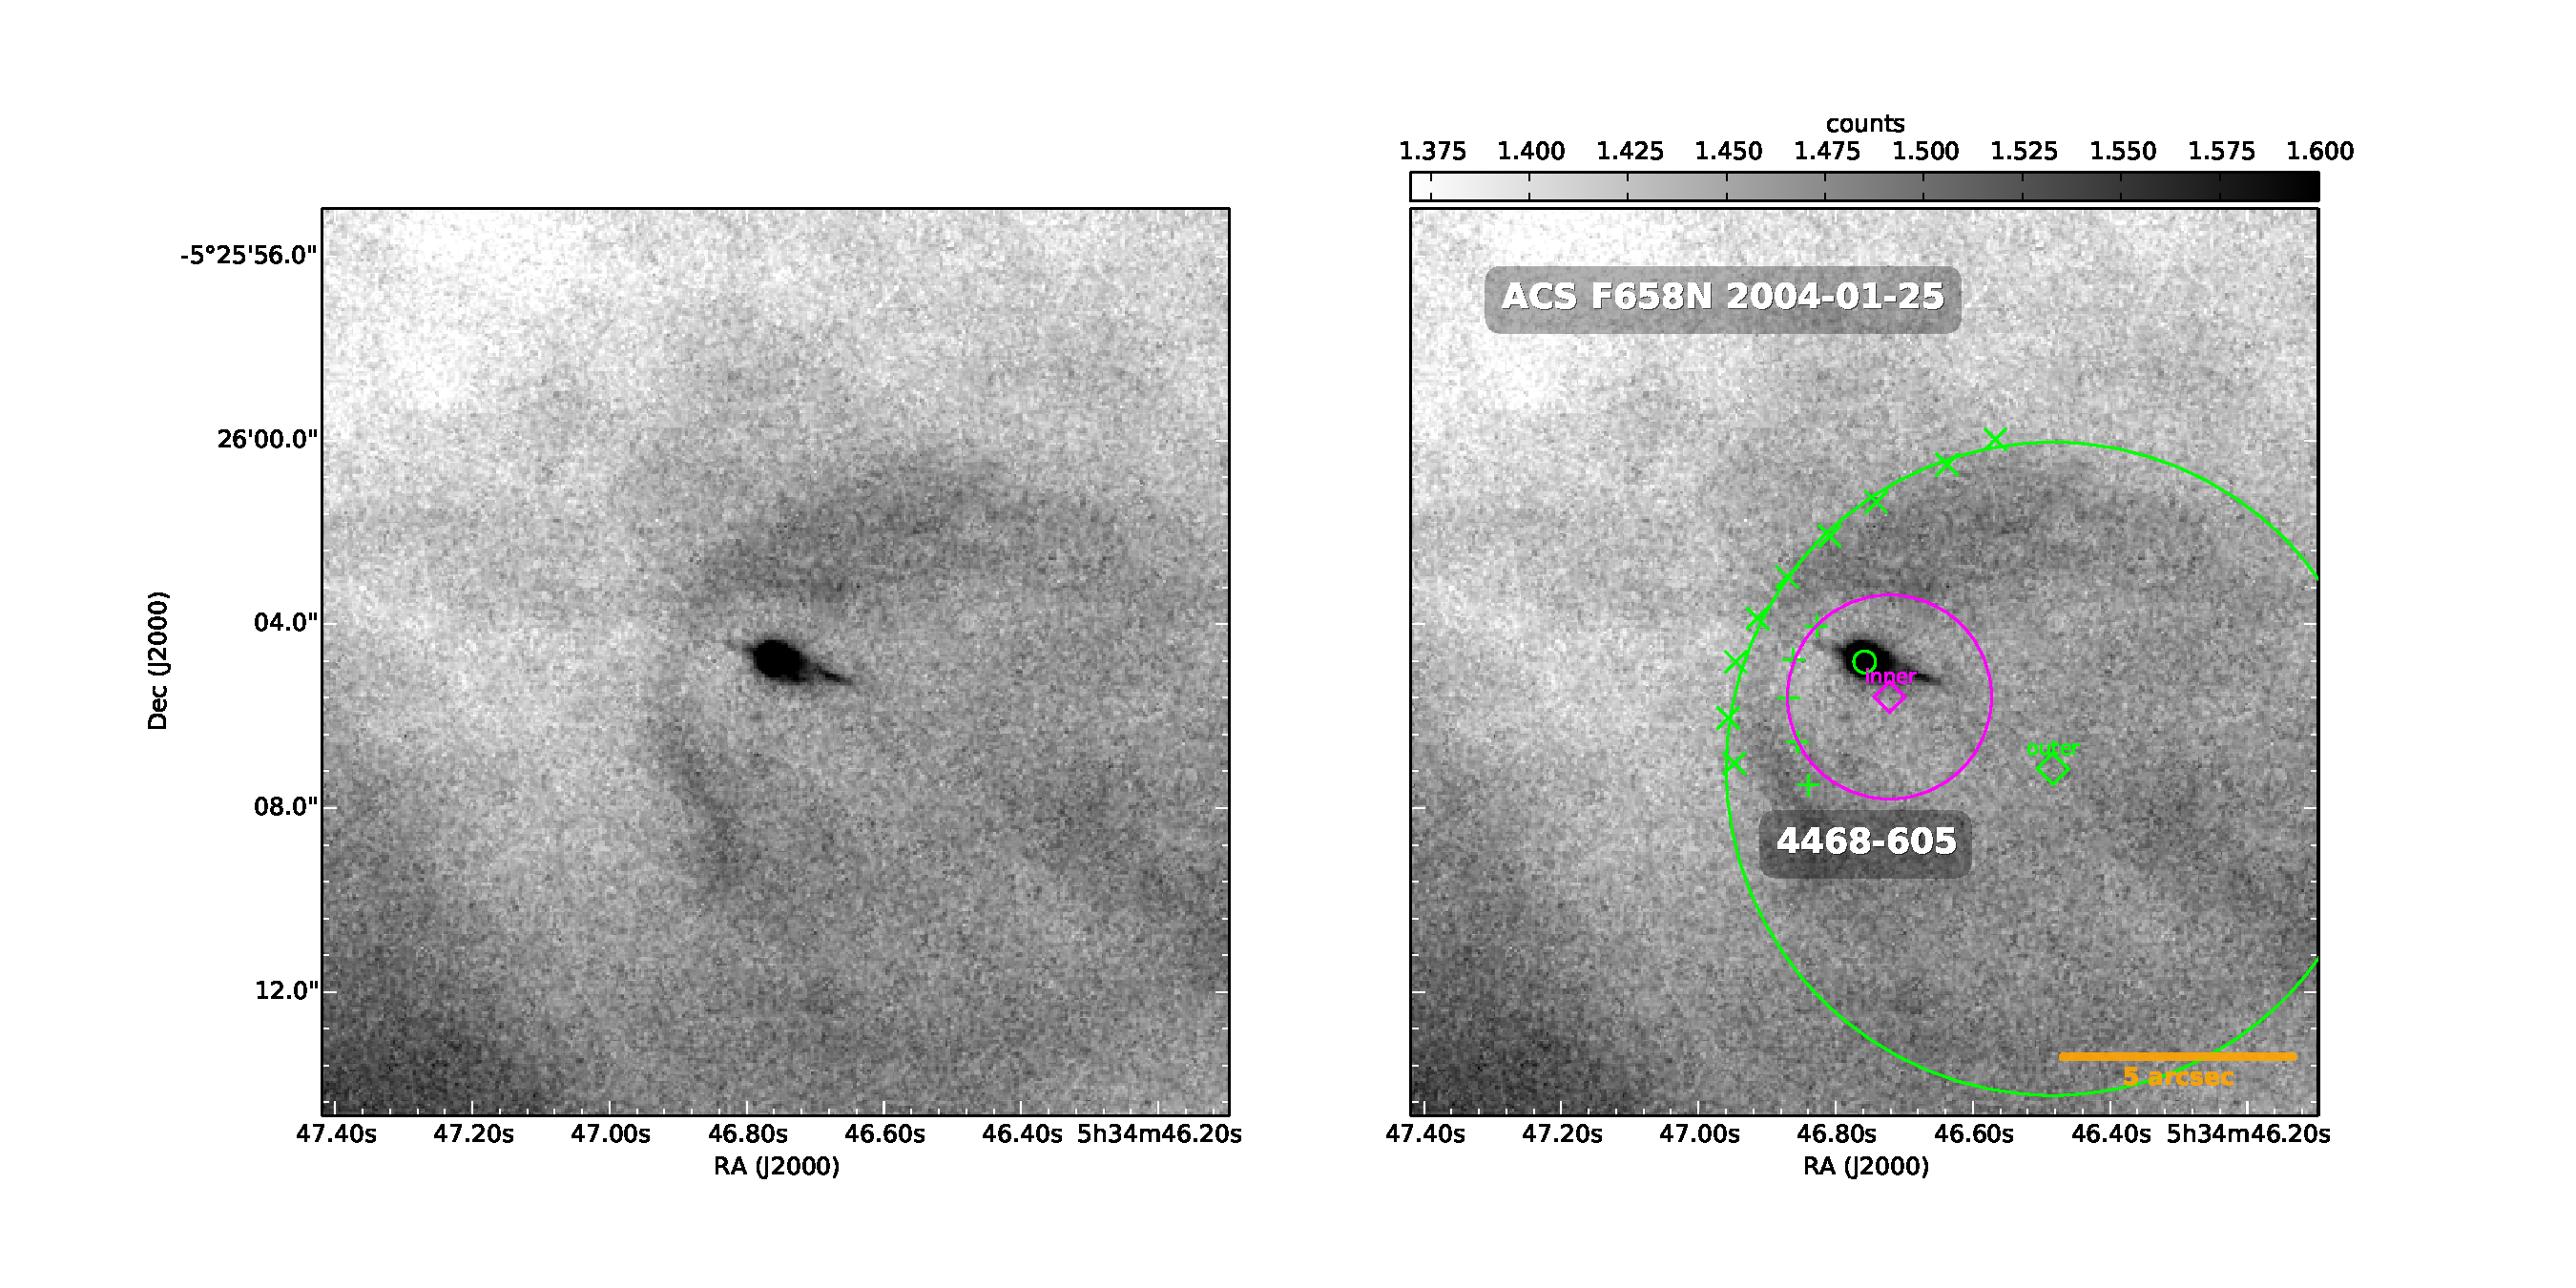
\includegraphics[width=0.5\linewidth]{./Figures/4468-605-Bally_17-images} &
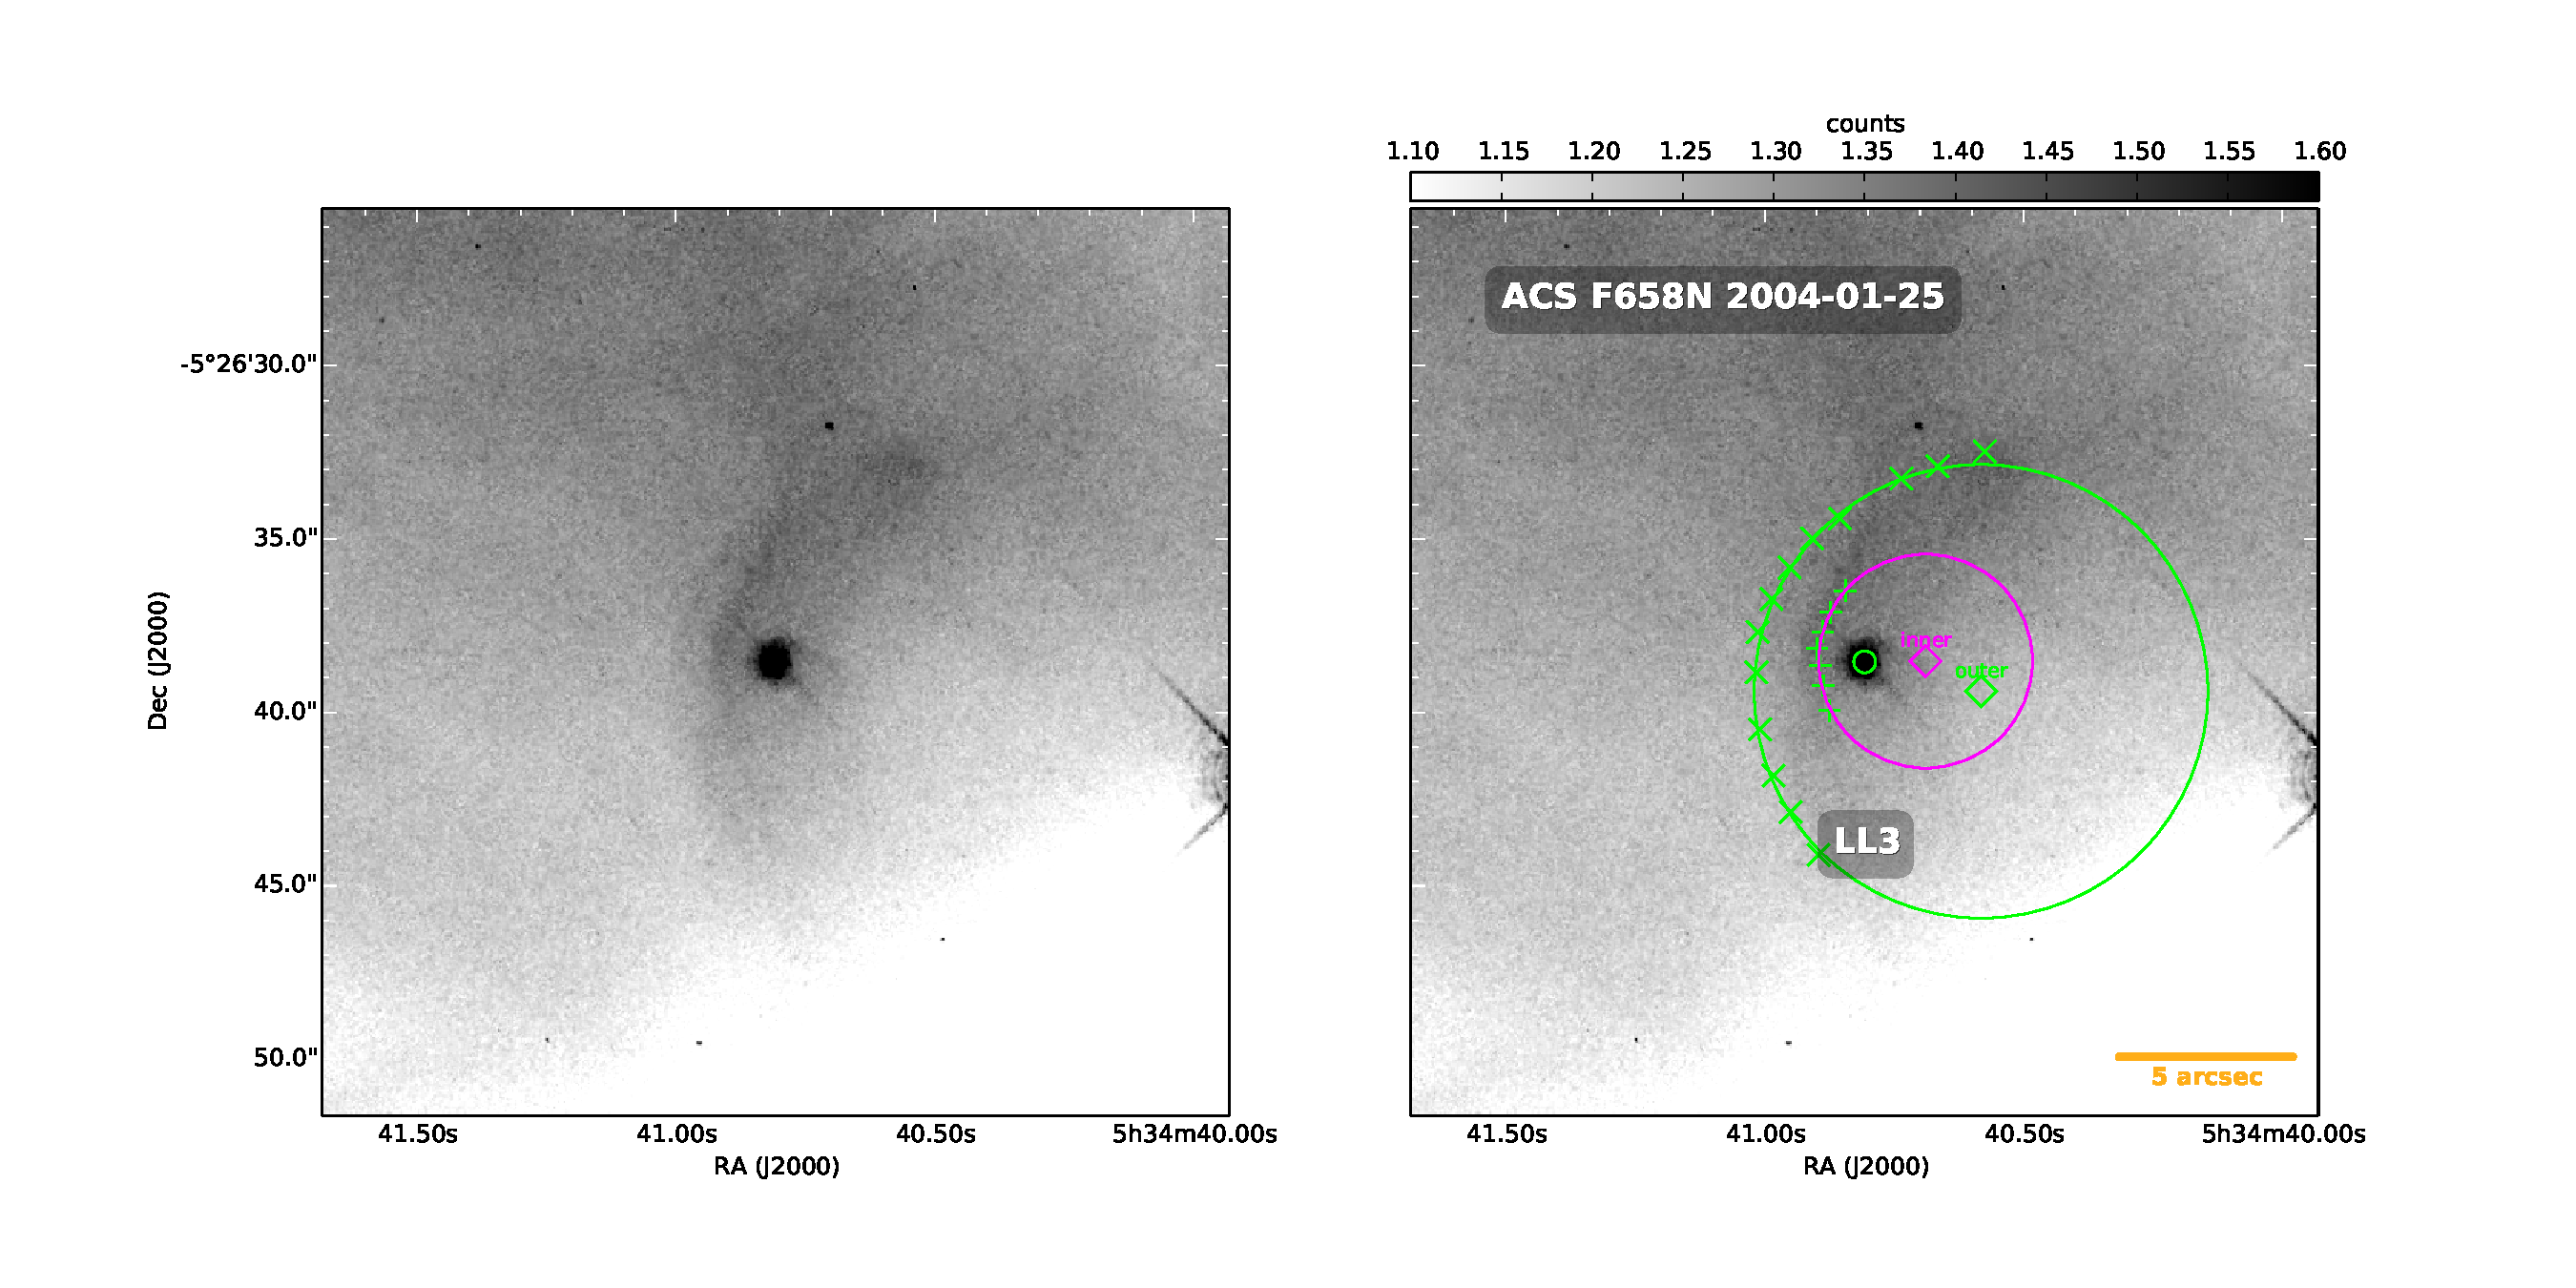
\includegraphics[width=0.5\linewidth]{./Figures/LL3-Bally_17-images}
  \end{tabular}
  \caption{}
  \label{fig:Luis-mosaic-2}
\end{figure}



\subsection{Mapa de Objetos}

A continuación mostramos el mapa de los objetos del catálogo de \citet{Gutierrez-Soto:2015a} dentro de la ONC.

\begin{figure}
  \begin{tabular}{cc}
    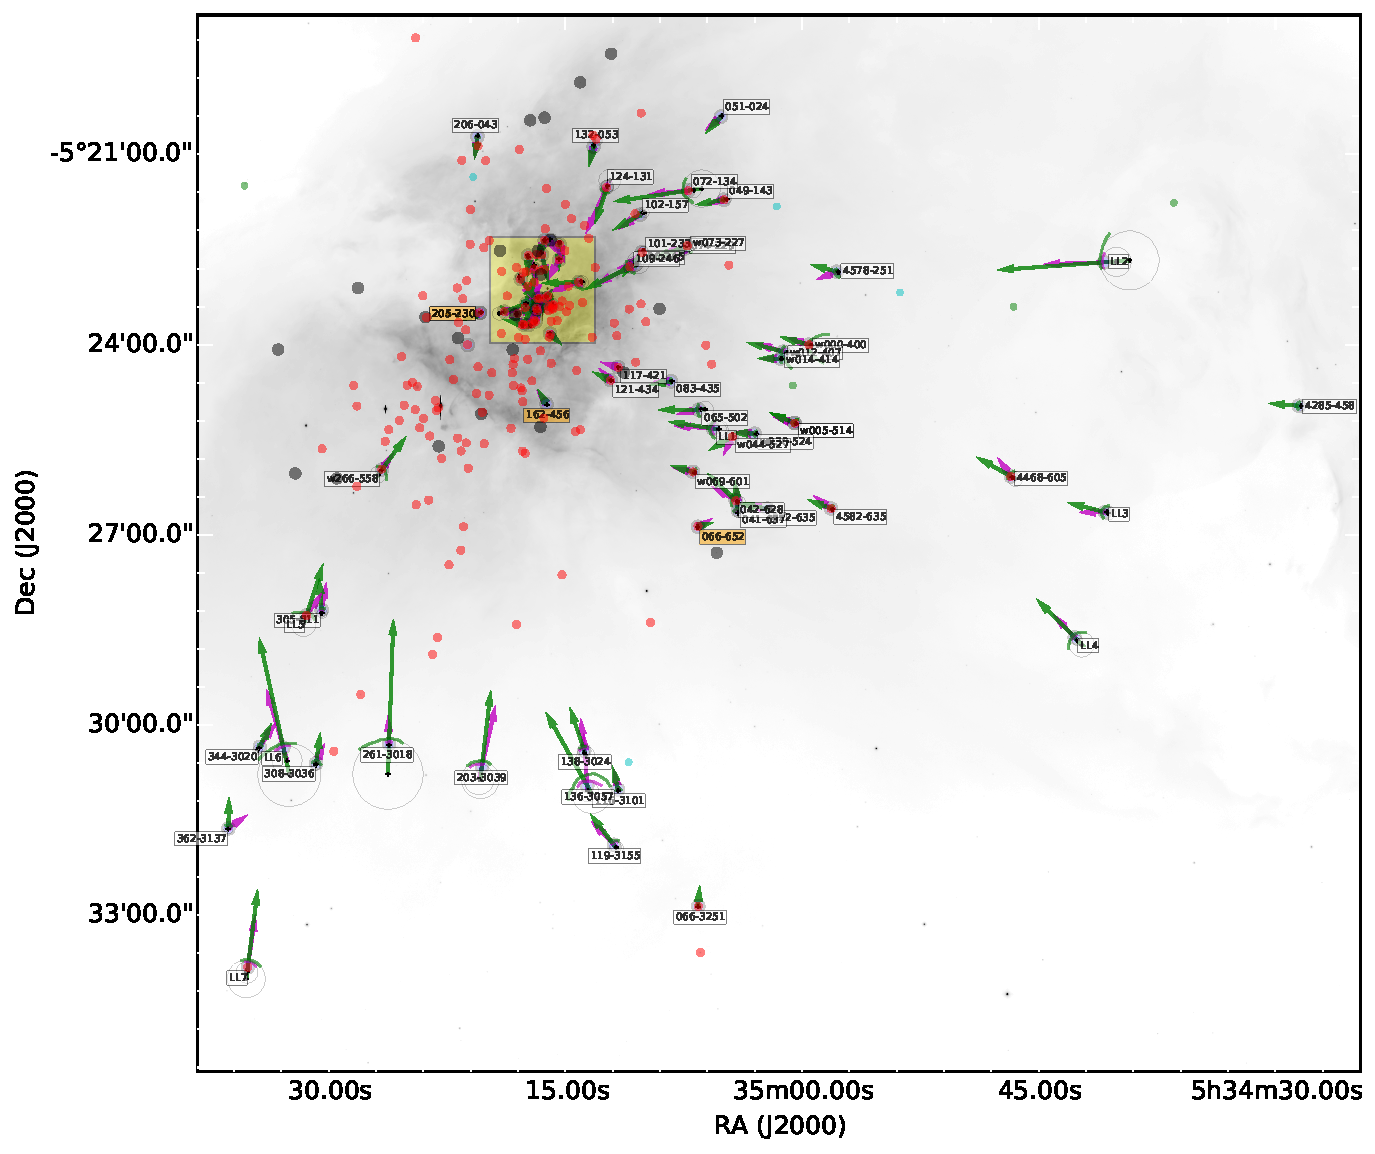
\includegraphics[width=0.5\linewidth]{./Figures/ll-pos-image-Luis} & 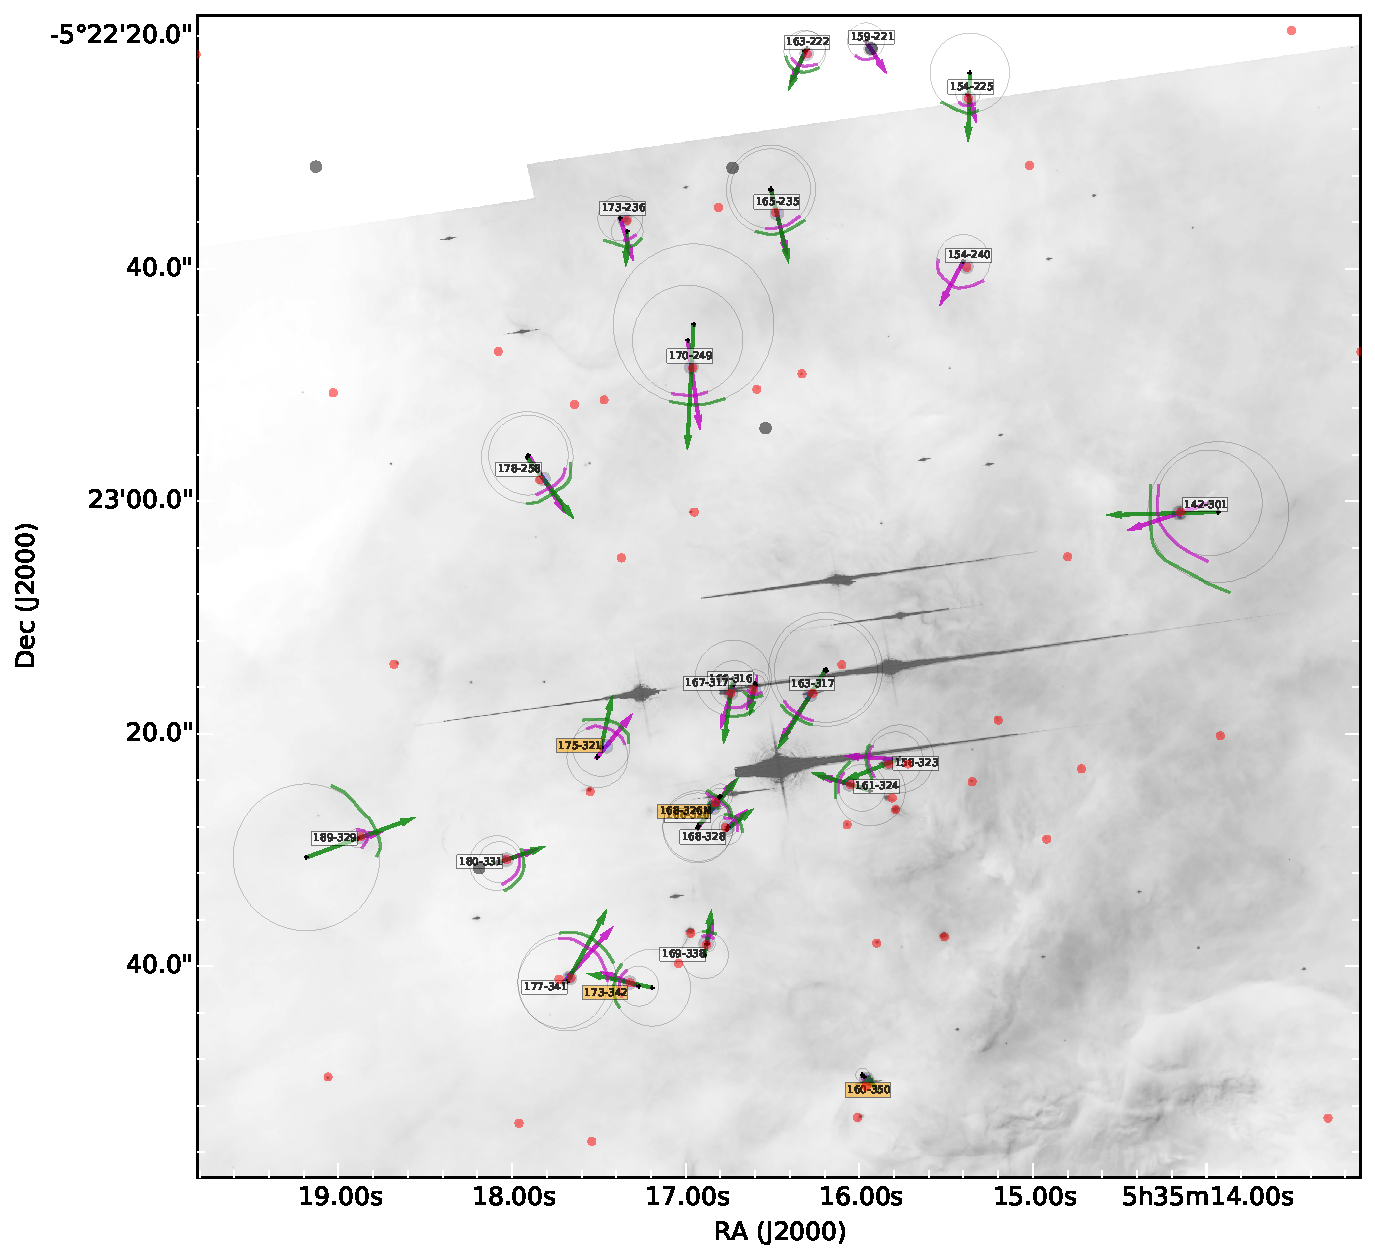
\includegraphics[width=0.46\linewidth]{./Figures/ll-pos-image-zoom-Luis}
  \end{tabular}
  \caption{Mapa de objetos del catálogo de \citet{Gutierrez-Soto:2015a} dentro de ONC. Las flechas de colores contienen la línea que une la posición del objeto central con el eje de curvatura de cada cáscara. Los puntos rojos representan objetos que no tienen un choque de proa visible. La zona marcada con el cuadrado amarillo se encuentra amplificada en el pánel derecho.}
  \label{fig:orion-map-LL}
\end{figure}


\section{Choques de Proa en el Medio Interestelar}

En general, un choque de proa se forma cuando un fluido interactua con un objeto moviéndose a velocidades supersónicas. Algunos ejemplos astrofísicos son:

\begin{itemize}
\item Superficies de trabajo de jets
\item Interacción de magnetósfera con el viento solar
\item Choques de proa estelares
  \begin{itemize}
  \item Estrellas AGB
  \item Estrellas O
  \item \textbf{Proplyds}
  \item Estrellas T Tauri
  \item Estrellas de Neutrones
  \end{itemize}
\end{itemize}

La morfología general de un choque de proa se ilustra en la figura \ref{fig:terminology}. La región donde la distancia entre el choque y la estrella (en el caso de un choque de proa \textit{estelar}) es la mínima, se denomina cabeza o \textit{ápex},mientras que las regiones más alejadas son denominadas las \textit{alas}. En el caso ideal los choques de proa son cilíndricamente simétricos.

\begin{figure}
  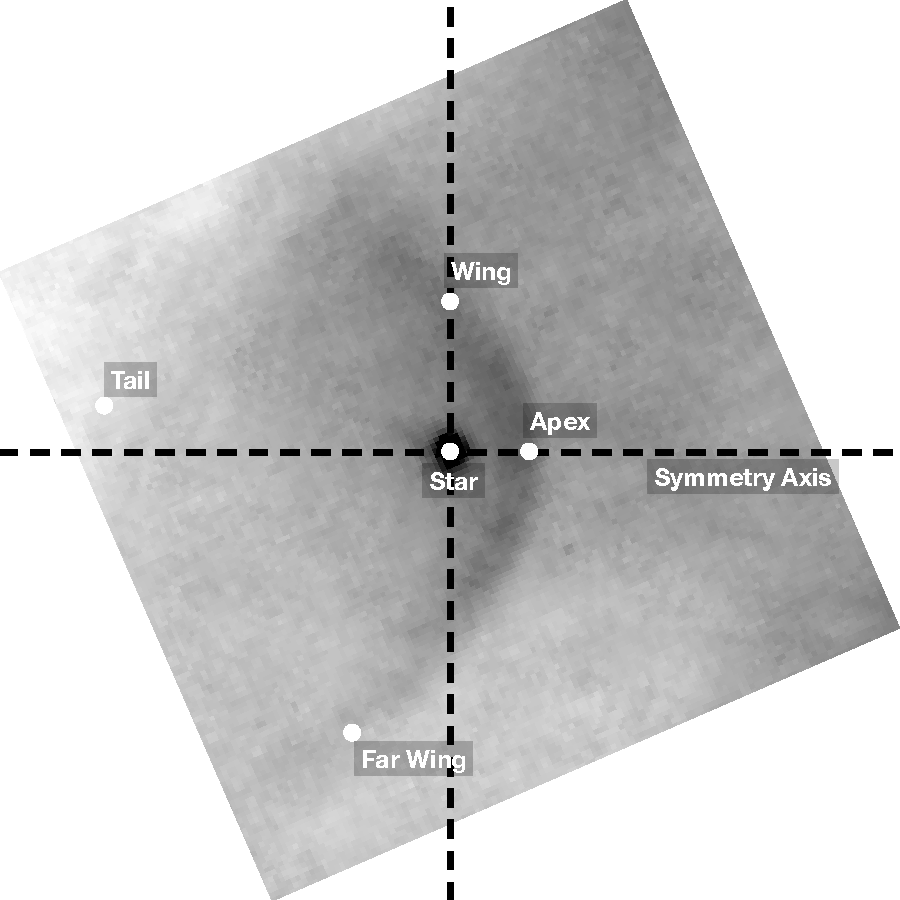
\includegraphics[width=0.7\linewidth]{./Figures/bow-terminology}
  \caption{Terminología de un choque de Proa}
  \label{fig:terminology}
\end{figure}

\subsection{Antecedentes}
Observaciones en mediano infrarrojo y en líneas de emisión de \Ion{H}{\alpha} y [\Ion{O}{III}] \citep{Robberto:2005, Bally:1998, Bally:2000} muestran de manera clara la presencia de arcos que rodean varios proplyds y otros objetos en la ONC cerca y lejos e la región del Trapecio. \citet{Hayward:1994} abre por primera vez la discusión acerca de la naturaleza de estos arcos (enfocándose en la región del Trapecio), sugiriendo que la presión de radiación y el viento estelar de \thC{} interactúan con el flujo de gas proveniente de cada proplyd individual.

\begin{figure}
  \begin{tabular}{lr}    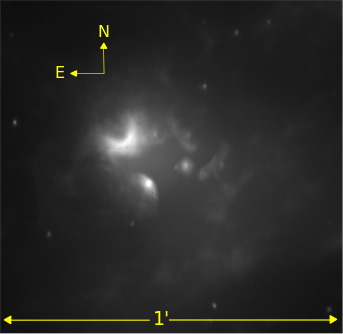
\includegraphics[width=0.5\linewidth]{./Figures/Orion_Robberto}&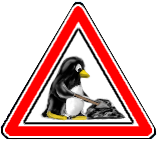
\includegraphics[width=0.1\linewidth]{./Figures/tux-development}
  \end{tabular}
  \caption{La región del trapecio en \SI{10}{\mu m}. \thC{} es la fuente débil al centro de la imagen. Dentro de este campo además se encuentran los proplyds LV1-LV5 con sus respectivos arcos. Al noreste se encuentra una fuente extensa llamada la Nebulosa Ney Allen (NA). El norte es encuentra hacia arriba y el este a la izquierda. El tamaño del campo es de aproximadamente $1' \times 1'$ \citep{Robberto:2005}.}
\end{figure}

Asimismo, en \citet{Robberto:2005} se hicieron mediciones de la forma de estos arcos, utlizando el radio aparente en el ápex $R_0/D$ y el radio perpendicular a éste $R_{90}/D$ (la alatud en este trabajo, excepto que normalizada con la distancia a \thC{} $D$, ver \S \ref{sec:char-rad}) para los proplyds LV1-LV5 y la nebulosa Ney-Allen, y los compararon con el modelo de capa delgada \citep{Canto:1996} (figura \ref{fig:Robberto}). Encontraron que aunque los proplyds LV1, LV4 y posiblemente LV5 ajustan a dicho modelo, pero el resto se aleja mucho de las curvas teóricas. Ésto no se puede atribuir atribuir a las limitaciones de la aproximación algebraica hecha por \citet{Canto:1996}, debido a que aun con todas las simplificaciones que conlleva, ajusta bien con modelos hidrodinámicos más complejos \citep{Garcia-Arredondo:2001}. Este trabajo es en parte la inspiración para esta tesis, ya que para explicar la discrepancia en la figura \ref{fig:Robberto} con los proplyds restantes nos llevó a extender el modelo de \citet{Canto:1996} al caso donde el viento interior no es isotrópico.

\begin{figure}
  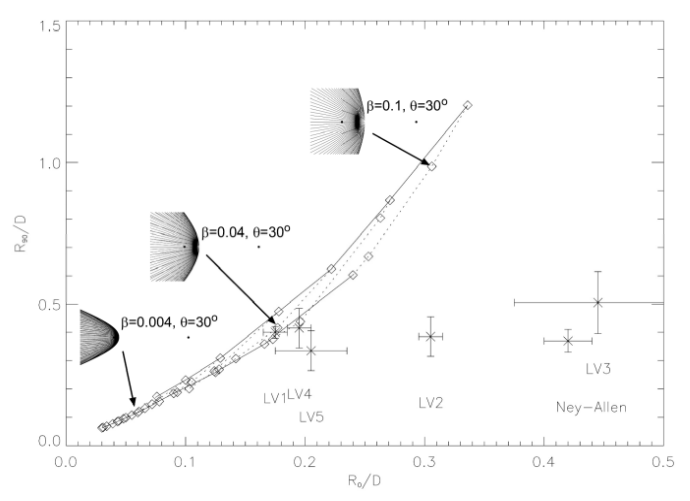
\includegraphics[width=0.7\linewidth]{./Figures/robberto}
  \caption{Comparación de los Radio Característicos aparentes $R'_{90}/D$ y $R_0/D$ para los proplyds LV1-LV5 y para la Nebulosa Ney-Allen mostrados con puntos y sus respectivas incertidumbres, y los diamantes abiertos se muestran soluciones al modelo de capa delgada de \citep{Canto:1996} para $\beta=[0.001, 0.002, 0.004, 0.01, 0.02, 0.1]$ y para intervalos de inclinaciones de $15^\circ$ entre $0^\circ$ y la inclinación máxima (ver \S \ref{sec:fundamental-parameters}, \ref{projection}).}
  \label{fig:Robberto}
\end{figure}

\begin{figure}
  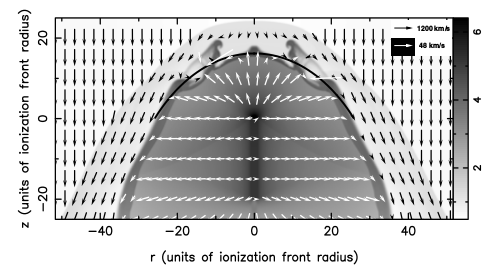
\includegraphics[width=0.7\linewidth]{./Figures/GA-simulation}
  \caption{Resultado de una simulación hidrodinámica de la interacción de un flujo fotoevaporado de un proplyd con un viento estelar. Las flechas indican la velocidad de los flujos (negro para el viento estelar y blanco para el flujo fotoevaporado del proplyd) y la escala gris representa el logaritmo de la densidad. Los ejes están en coordenadas cilíndricas $(r, z)$ en unidades del radio del IF. El arco negro representa la solución analítica de la posición de la discontinuidad de contacto de un choque ancantoide con $k=1/2$ y $\beta=0.002$ \citep{Garcia-Arredondo:2001}}
  \label{fig:simulation}
\end{figure}

\subsection{Estrellas ``Errantes''}

Otro tipo de choques de proa estelares ocurren cuando los vientos de estrellas \textit{errantes} (runaway stars), usualmente de tipos espectrales OB, con velocidades de $ >\SI{30}{km.s^{-1}}$ interactúan con el medio interestelar \citep{Kobulnicky:2016}. Estas estrellas adquieren estas velocidades cuando sufren encuentros dinámicos cercanos dentro del cúmulo donde se formaron o bien cuando forman parte de un sistema binario cerrado y uno de los miembros explota como supernova.

En la figura \ref{fig:runaway} se muestran algunos ejemplos típicos de choques de proa producidos por estrellas errantes. Los colores en cada imagen representan a la banda de \SI{24}{\mu.m} del Telescopio Espacial Spitzer, o bien la de \SI{22}{\mu.m} del catálogo WISE para el color rojo, para el color verde puede ser la banda de \SI{8}{\mu.m} de Spitzer o la de \SI{12}{\mu.m} de WISE, y al color azul le corresponde la banda de \SI{4.5}{\mu.m} de Spitzer o WISE y los objetos mostrados son, de arriba a abajo y de izquierda a derecha: $\zeta$\,Oph, AE Aur, HD136003, HD150898, HD155755 y HD143275, y por último, la flecha blanca indica la magnitud y dirección del movimiento propio de la estrella.

\begin{figure}
  \centering
  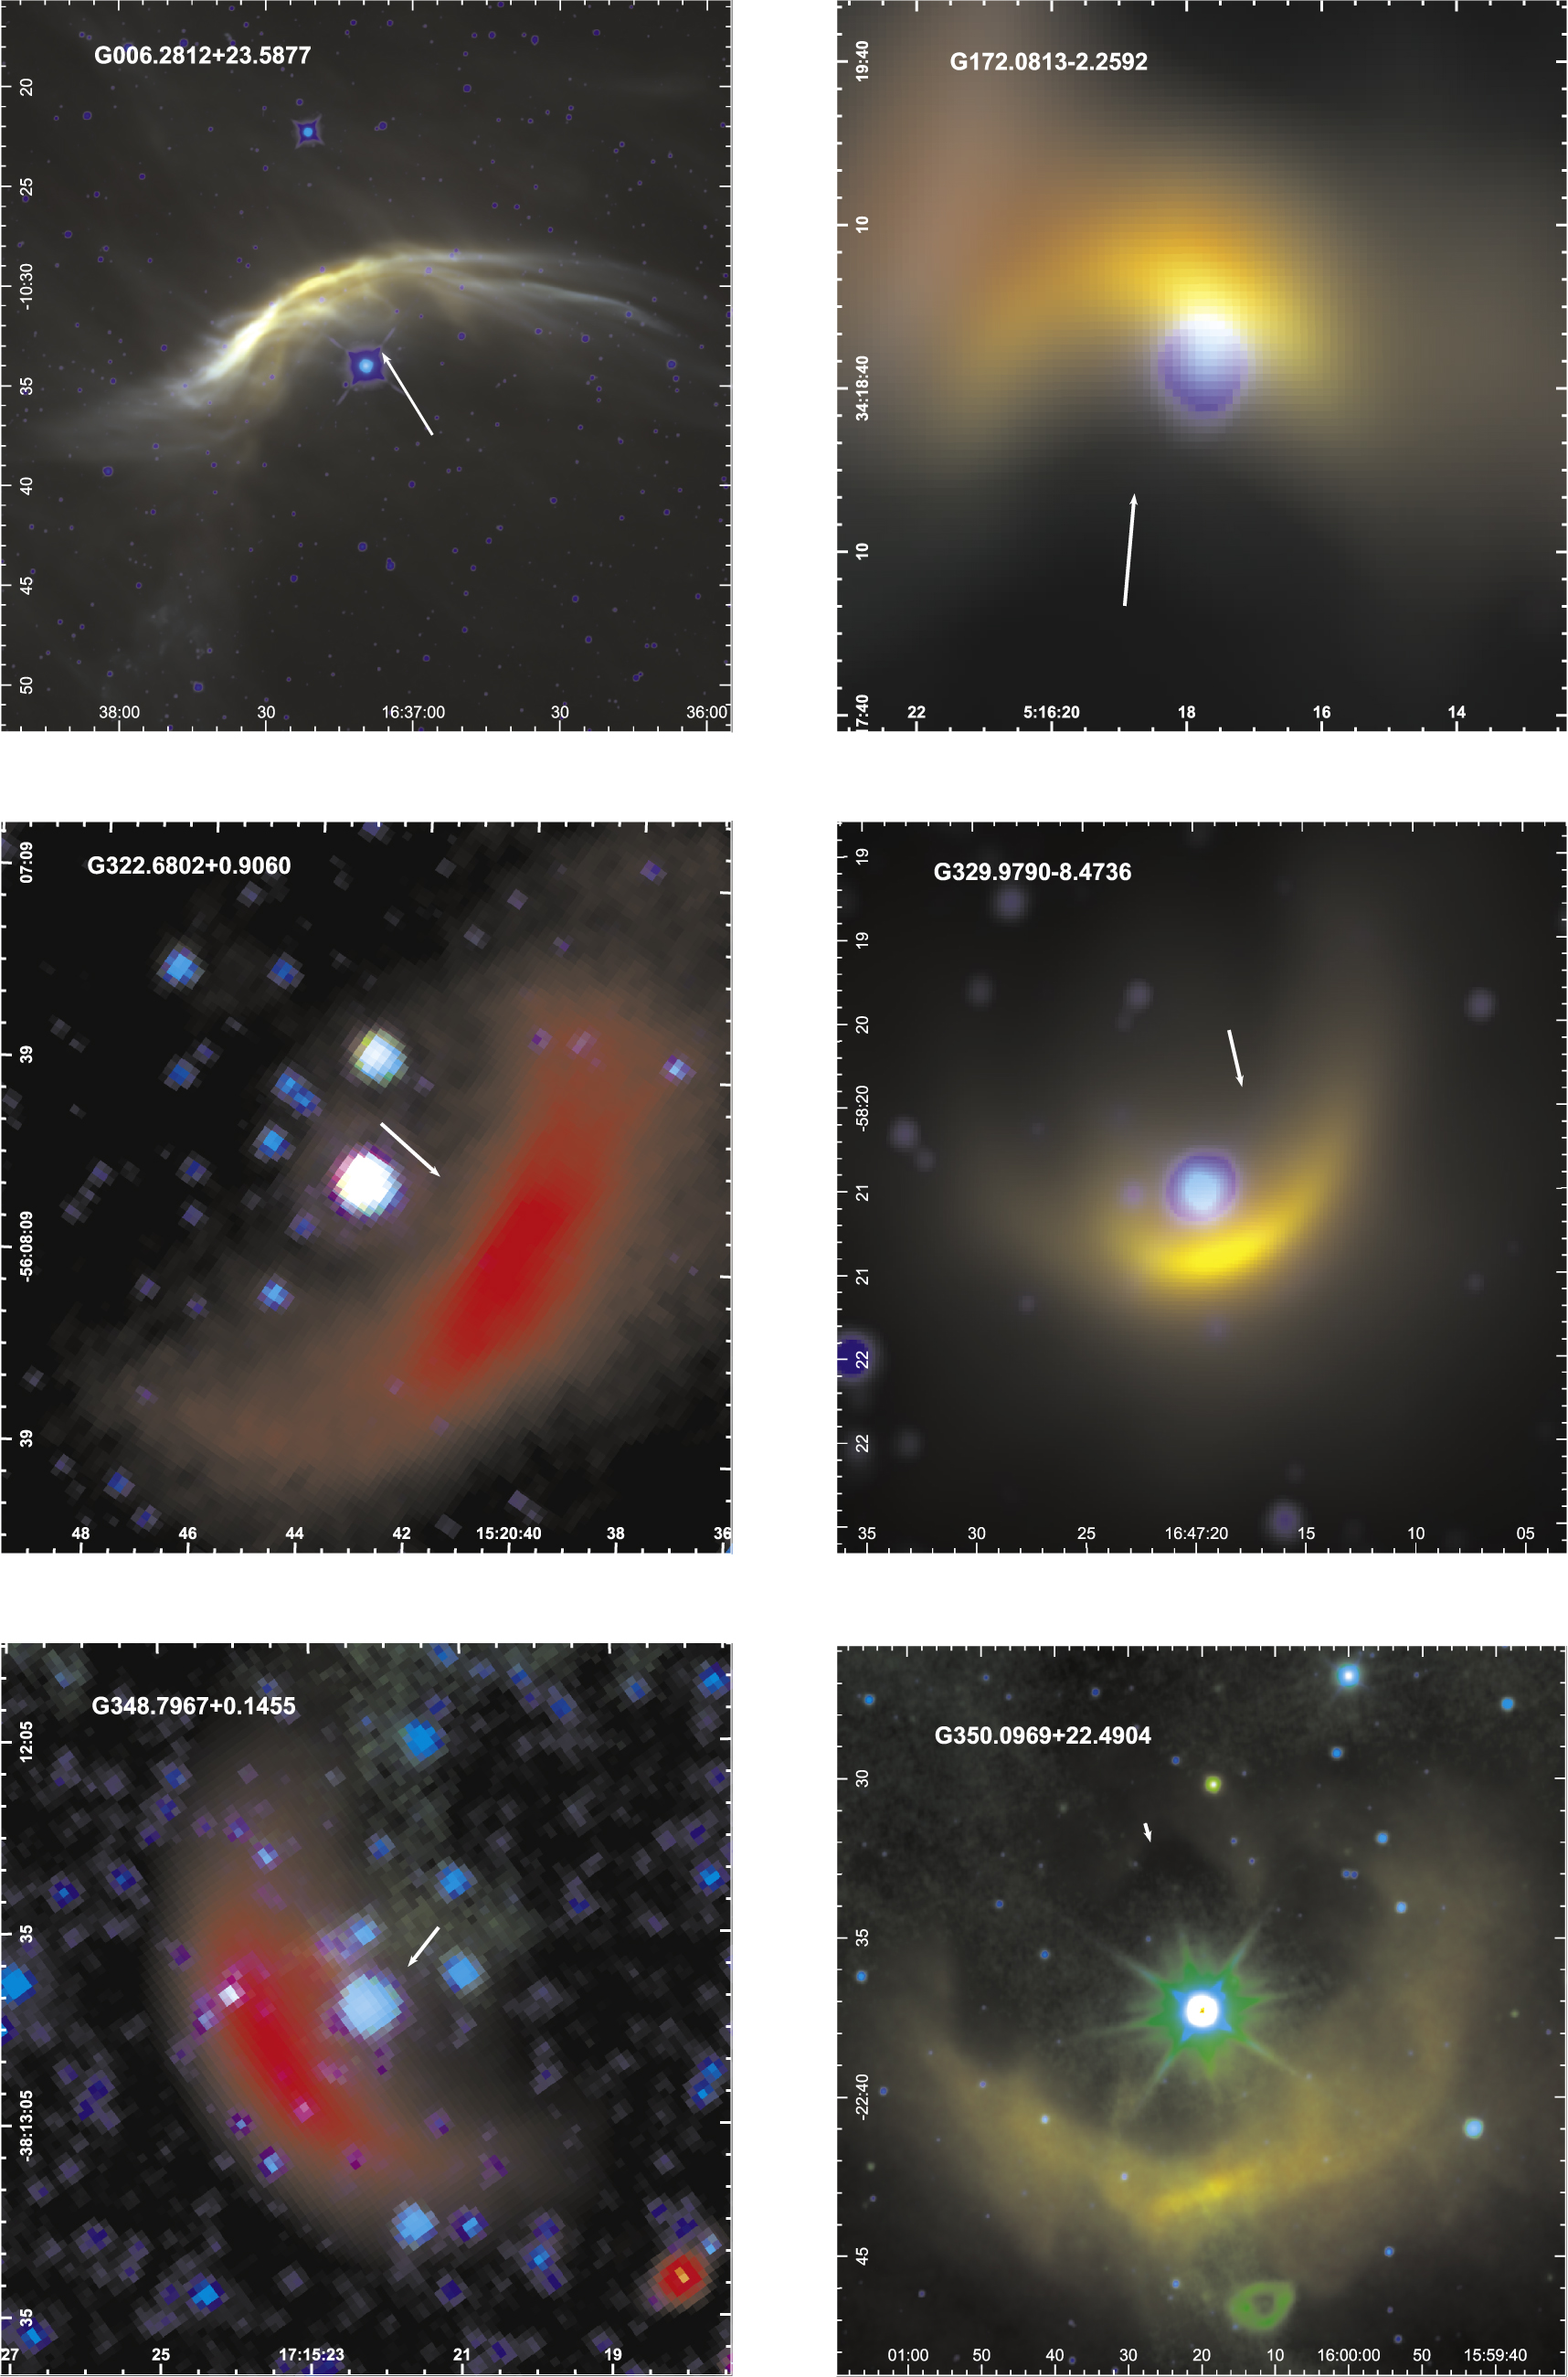
\includegraphics[width=0.7\linewidth]{./Figures/kobulnicky}
  \caption{Ejemplos de choques de proa en infrarrojo producidos por estrellas errantes, tomados por el telescopio espacial Spitzer o del catálogo WISE. Los colores representan las bandas de \SI{24}{\mu.m} de Spitzer o \SI{22}{\mu.m} de WISE (rojo), \SI{8}{\mu.m} de Spitzer o \SI{12}{\mu.m} de WISE (verde) y \SI{4.5}{\mu.m} de de Spitzer o WISE (azul). Los objetos mostrados son: $\zeta$\, Oph (G006.2812+23.5877; arriba izquierda), AE Aur (G172.0813-02.2592; arriba derecha), HD136003 (G322.6802+00.9060; centro izquierda), HD150898 (G329.9790-08.4736; centro derecha), HD155755 (G348.7967+00.1455; abajo izquierda) y HD143275 (G350.0969+22.4904; abajo derecha). La magnitud y dirección del movimiento propio se muestra con las flechas blancas \citep{Kobulnicky:2016}.}
  \label{fig:runaway}
\end{figure}

\subsection{Estrellas AGB y Supergigantes Rojas}

Otro tipo de choques de proa estelares se forma cuando estrellas en sus fases evolutivas finales, tales como estrellas AGB y supergigantes rojas pierden material a través de fuertes vientos que producen choques al interaccionar con el Medio Interestelar \citep{Cox:2012}.

En la figura  \ref{fig:fermata} se muestran ejemplos de estrellas AGB y supergigantes en infrarrojo lejano que forman parte del programa MESS (Mass-loss of Evolved StarS, \citet{Groenewegen:2011}) que utilizan el instrumento PACS (Photodetector Array Camera Spectrometer), donde se usan los filtros de \SI{70}{\mu.m} y \SI{160}{\mu.m}, y que muestran choques tipo ``fermata''. Otras formas que se observan son tipo ``ojos'', ``anillos'' e ``irregulares'' (ver tabla \ref{tab:morphology-AGB}).

\begin{figure}
  \centering
  \includegraphics[width=0.5\linewidth]{./Figures/Cox-fermata}
  \caption{Interacciones tipo ``fermata'' de los objetos R\,Scl, NML\,Tau, W\,Ori, W\,Pic y $\alpha$\,Ori tomadas con PACS en los filtros de \SI{70}{\mu.m} (izquierda) y \SI{160}{\mu.m} (derecha). La barra blanca mide 1' en la imagen, así como su respectivo tamaño físico. En todos los páneles el norte se ubica hacia arriba y el este a la izquierda. La línea negra indica la velocidad y dirección de la velocidad espacial de la estrella, adoptando una escala tal que \SI{1}{km.s} corresponde a 1'' en la imagen \citep{Cox:2012}. Nota adicional. R\,Scl tiene una cáscara esférica interna no visible en la imagen.}
  \label{fig:fermata}
\end{figure}

\begin{table}
  \begin{tabular}{llc}
    \toprule
    Clase & Descripción & Forma \\
    \midrule
    I & Fermata & 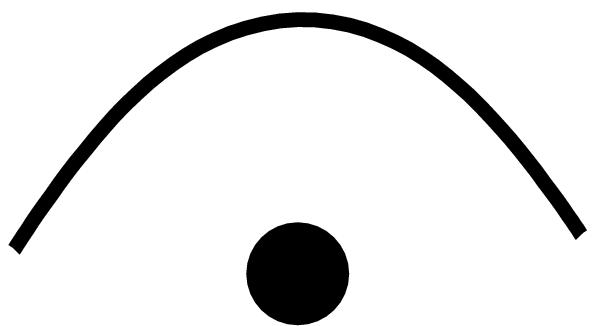
\includegraphics[scale=0.03]{./Figures/fermata} \\
    II & Ojos   & 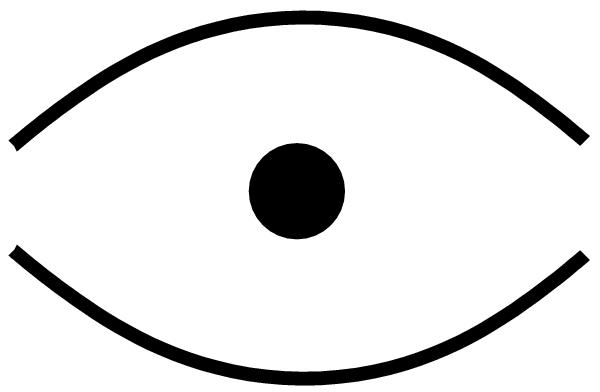
\includegraphics[scale=0.03]{./Figures/eyes} \\
    III & Anillos & 
\includegraphics[scale=0.02]{./Figures/ring} \\
    IV & Irregulares & \\
    \bottomrule
  \end{tabular}
  \caption{Clasificación morfológica de choques de proa estelares de estrellas AGB y supergigantes \citep{Cox:2012}.}
  \label{tab:morphology-AGB}
\end{table}


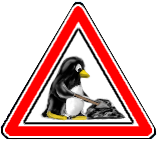
\includegraphics[width=0.1\linewidth]{./Figures/tux-development}
